%% Placeholder for chapter on linear, quadratic, and geometric models

\section{Linear Programs: An Optimization Problem}

Also known as(a.k.a) (mathematical program") of the form

\begin{align*}
(arg)\,\,min_{x\in \Re^n}&c^Tx + d\,\,\,\text{("objective"function)}\\
s.t.\,\,\, &Ax = b\\
&Gx \leq h
\end{align*}

"Feasible" set(might not be good idea, but you can do this): $S = \{x|Ax = b, Gx \leq h \}$


\begin{itemize}
	\item $c\in \Re^n$, $d\in \Re$.
	
	\item $A\in \Re^{q\times n}$, $b\in \Re^q$, \begin{equation*}
	A = 
	\begin{bmatrix}
	\alpha^{(1)^T}\\
	...\\
	\alpha^{(q)^T}
	\end{bmatrix}
	\end{equation*}
	
	$<\alpha^{(i)}, x> =b_i$, $i\in \left[q\right]$
	
	\item $G\in \Re^{m\times n}$, $h\in \Re^m$
	
	\item If
	\begin{equation*}
	G = 
	\begin{bmatrix}
	g^{(1)^T}\\
	...\\
	g^{(q)^T}
	\end{bmatrix}
	\end{equation*}
	
	Then $<G^{(i)}, x>\leq h_i$, $i\in \left[m\right]$
	
\end{itemize}





\begin{align*}
p^* = min \,\,\, &c^Tx + d\\
s.t.\,\,\, &Ax = b\\
&Gx\leq h
\end{align*}

"optimal" value of program:

\begin{itemize}
	\item Lowest cost shoice amongst all feasible $x$.
	
	\item Possible here is no minimal choice
	
	\item possible no feasible choice
	
	\item $p^*\in \Re$
\end{itemize}


\begin{align*}
x^* = min \,\,\, &c^Tx + d\\
s.t.\,\,\, &Ax = b\\
&Gx\leq h
\end{align*}

$x^*$ "optimal" choice of optimization variable(or vector):

\begin{itemize}
	\item sometimes $x^*$ does not exist
	
	\item if exists, may or may not be unique
	
	\item $x^*\in \Re^n$
\end{itemize}


Let's consider an example:\\

During the The Second World War, the US army is considering how to make their soldiers have enough nutrients...\\

Different nutrients in different foods and daily requirement:\\


\begin{tabular}{|c|c|c|c|}
	\hline 
	Nutrients&Meat&Potatoes&Daily Requirement\\
	\hline  
	Carbohydates&40&200&400\\
	\hline  
	Protein&100&20&200\\
	\hline  
	Fiber&5&40&40\\
	\hline 
\end{tabular}\\

The price of meat and potatoes:\\



\begin{tabular}{|c|c|}
	\hline 
	Resources&cost/kg\\
	\hline  
	Meat &\$ 1\\
	\hline 
	Potatoes &\$ 0.25\\
	\hline 
\end{tabular}

$x_1$ denotes meat(kg) and $x_2$ denotes potatoes(kg).\\


Objective:

\begin{equation*}
x_1 + \frac{1}{4}x_2 = 
\begin{bmatrix}
1 & \frac{1}{4}
\end{bmatrix}
\begin{bmatrix}
x_1\\
x_2
\end{bmatrix}
\end{equation*}

Constrains:
\begin{align*}
40x_1 + 200x_2 &\geq 400\\
100x_1 + 20x_2 &\geq 200\\
5x_1 + 40x_2 &\geq 40\\
x_1 \geq 0\\
x_2 \geq 0
\end{align*}

$Gx\leq h \rightarrow$ 

\begin{equation*}
\begin{bmatrix}
-\frac{1}{5} & -1\\
-\frac{1}{8} & -1\\
-5 & -1\\
-1 & 0\\
0 & -1
\end{bmatrix}
\begin{bmatrix}
x_1\\
x_2
\end{bmatrix}\leq
\begin{bmatrix}
-2\\
-1\\
-10\\
0\\
0
\end{bmatrix}
\end{equation*}

\begin{figure}
	\centering
	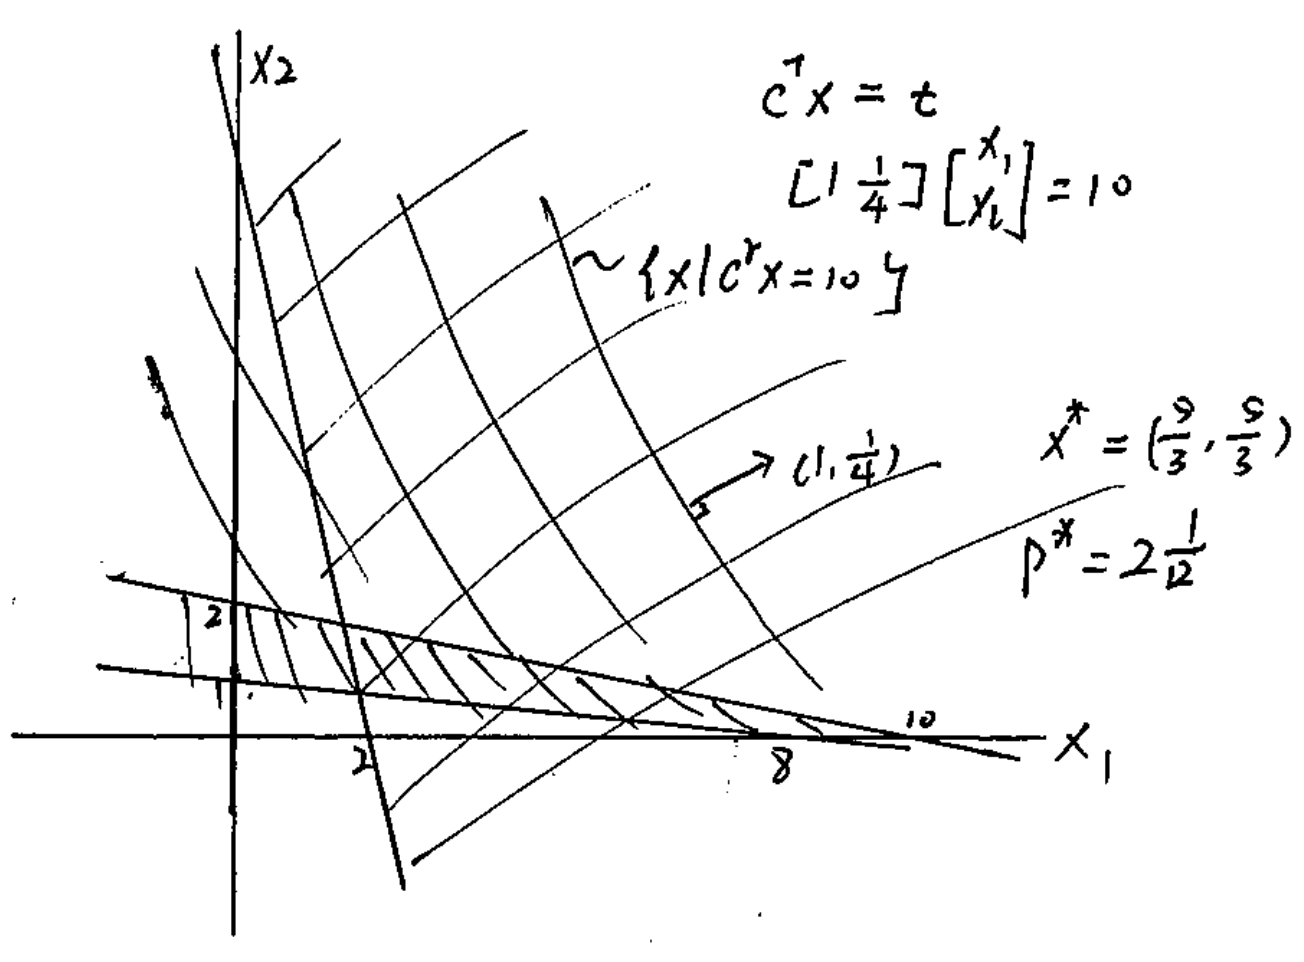
\includegraphics[width=2.1in,height=2.1in]{figures/ch06/figure5.png}
	%\caption{This is an inserted JPG graphic} 
	%\label{fig:graph} 
\end{figure}

%Below are notes for Oct 12
We have started talking about Linear Programming problems:

\begin{align*}
(arg)min_{x\in \Re^n} \,\,\, c^Tx + d\\
s.t. \,\,\, Ax& = b\\
Gx &\leq h\\
A&\in \Re^{q\times n}, b\in \Re^{q}\\
G&\in \Re^{m\times n}, h\in \Re^{m}
\end{align*}

Objective of LP, have or don't have constraints

\begin{align*}
p^* &= min \,\,\, c^Tx+d\\
x^* &= arg\,\, min_{x\in \Re^n} \,\,\, c^Tx+d
\end{align*}

Probability 1: $c = 0 \in \Re^n$

\begin{align*}
p^* &= min_{x\in \Re^n} \,\,\, d=d\\
x^* &= arg\,\, min_{x\in \Re^n} \,\,\, d = \Re^n
\end{align*}

Probability 2: $c \neq 0 \in \Re^n$

\begin{align*}
p^* &= -\infty\,\,\, \text{by convention if no minimum}\\
x(\alpha) &= -\alpha c \,\,\, \alpha \geq 0\\
c^Tx + d &= c^T(-\alpha c) + d = \alpha - \alpha c^Tc = \alpha - \alpha||c||^2_2\\
x^* &\text{doesn't exist}
\end{align*}

So for unconstrained LP:

\begin{equation*}
%\label{eq6}
p^*=\left\{
\begin{aligned}
d &  & \text{if } c=0 \\
-\infty &  & \text{otherwise}
\end{aligned}
\right.
\end{equation*}

\begin{equation*}
%\label{eq6}
x^*=\left\{
\begin{aligned}
\Re^n & &\text{if } c=0 \\
\text{doesn't exist} &  & \text{otherwise}
\end{aligned}
\right.
\end{equation*}

Think about geometry of cost function:

\begin{equation*}
F_0(x)(\text{"objective function"}) =c^Tx + d(affine function)
\end{equation*}

\begin{align*}
c_{F_0}(t) &= x\in \Re^n | F_0(x) = c^Tx + d = t \}(\text{hyper-plane})\\
&= \{x\in \Re^n | C^Tx = (t-d) \}(\text{offset when t=d}, C_{F_0}(t) \text{is a subspace})
\end{align*}

\begin{figure}
	\centering
	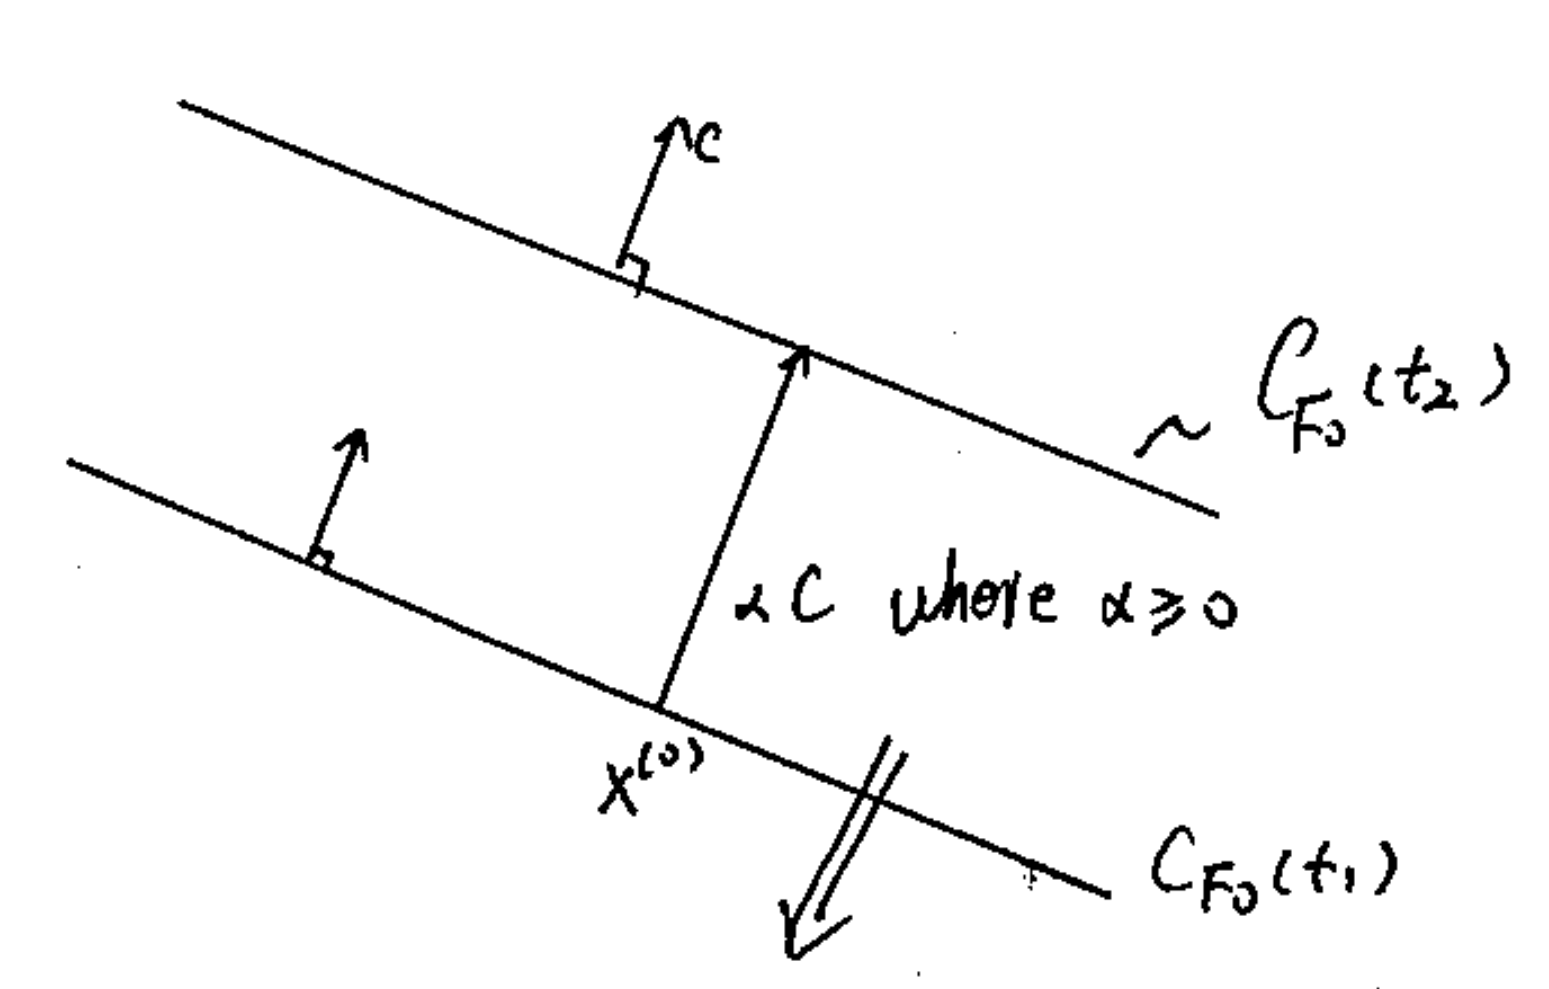
\includegraphics[width=2.1in,height=2.1in]{figures/ch07/figure1012_1.png}
	%\caption{This is an inserted JPG graphic} 
	%\label{fig:graph} 
\end{figure}

To find the relationship between $t_1$ and $t_2$:

\begin{align*}
t_2 &= c^T(x^{(0)}+\aleph c) + d\\
t_1 &= c^Tx^{(0)} + d\\
t_2 - t_1 &= [c^Tx^{(0)} + d + \alpha ||c||^2] - c^Tx^{(0)} = \alpha \Vert c \Vert^2
\end{align*}

One approach:

%\begin{align*}
%t_2 &= c^T(x^{(0)} + \alpha c) + d\\
%t_1 &= c^Tx^{(0)} + d\\
%t_2 - t_1 &= \[c^Tx^{(0)} + d + \alpha||c||^2 \] - c^Tx^{(0)} + d\\
%&= \alpha ||c||^2\\
%\end{align*}

\begin{equation*}
\nabla F_0(x) =
	\begin{bmatrix}
	\frac{\sigma}{\sigma x_1}(c^Tx+d)\\
	\vdots\\
	\frac{\sigma}{\sigma x_n}(c^Tx+d)
	\end{bmatrix} = 
	\begin{bmatrix}
	c_1\\
	c_2\\
	\vdots\\
	c_n
	\end{bmatrix} = c
\end{equation*}

\begin{align*}
Ax &= b\\
Gx &\leq h
\end{align*}

Then it comes to:

\begin{equation*}
A = 
\begin{bmatrix}
\alpha^{(1)}\\
\alpha^{(2)}\\
\vdots\\
\alpha^{(q)}
\end{bmatrix}
\end{equation*}


\begin{equation*}
\{x|Ax = b \} =  \cap^q_{i=1}\{x|<\alpha^{(i)}, x> = b_i \}
\end{equation*}



The "feasible" set:

\begin{equation*}
S = \left(\cap^q_{i=1}\{x\in \Re^n | <\alpha^{(i)}, x> = b_i \}\right) \cap \left(\cap^m_{i=1}\{x\in \Re^n | <g^{(i)}, x> \leq h_i \}\right)
\end{equation*}

(Intersect half-spaces with hyper-planes)

\begin{itemize}
	\item "polyhedron" / "polytape"
	
	\item Ax = b $\rightarrow$ $Ax \leq b$, $Ax \geq b$
\end{itemize}

\begin{example}
	\begin{align*}A &= 
	\begin{bmatrix}
	1 & 1
	\end{bmatrix}
	b = 
	\begin{bmatrix}
	2
	\end{bmatrix}\\
	G &= 
	\begin{bmatrix}
	-1 & 0\\
	0 & -1
	\end{bmatrix}
	h = 
	\begin{bmatrix}
	0\\
	0
	\end{bmatrix}\\
	Ax &= b \rightarrow x_1 + x_2 = 2\\
	Gx &\leq h \rightarrow x_1 \geq 0, x_2\geq 0
	\end{align*}
	
	
	\begin{figure}
	\centering
	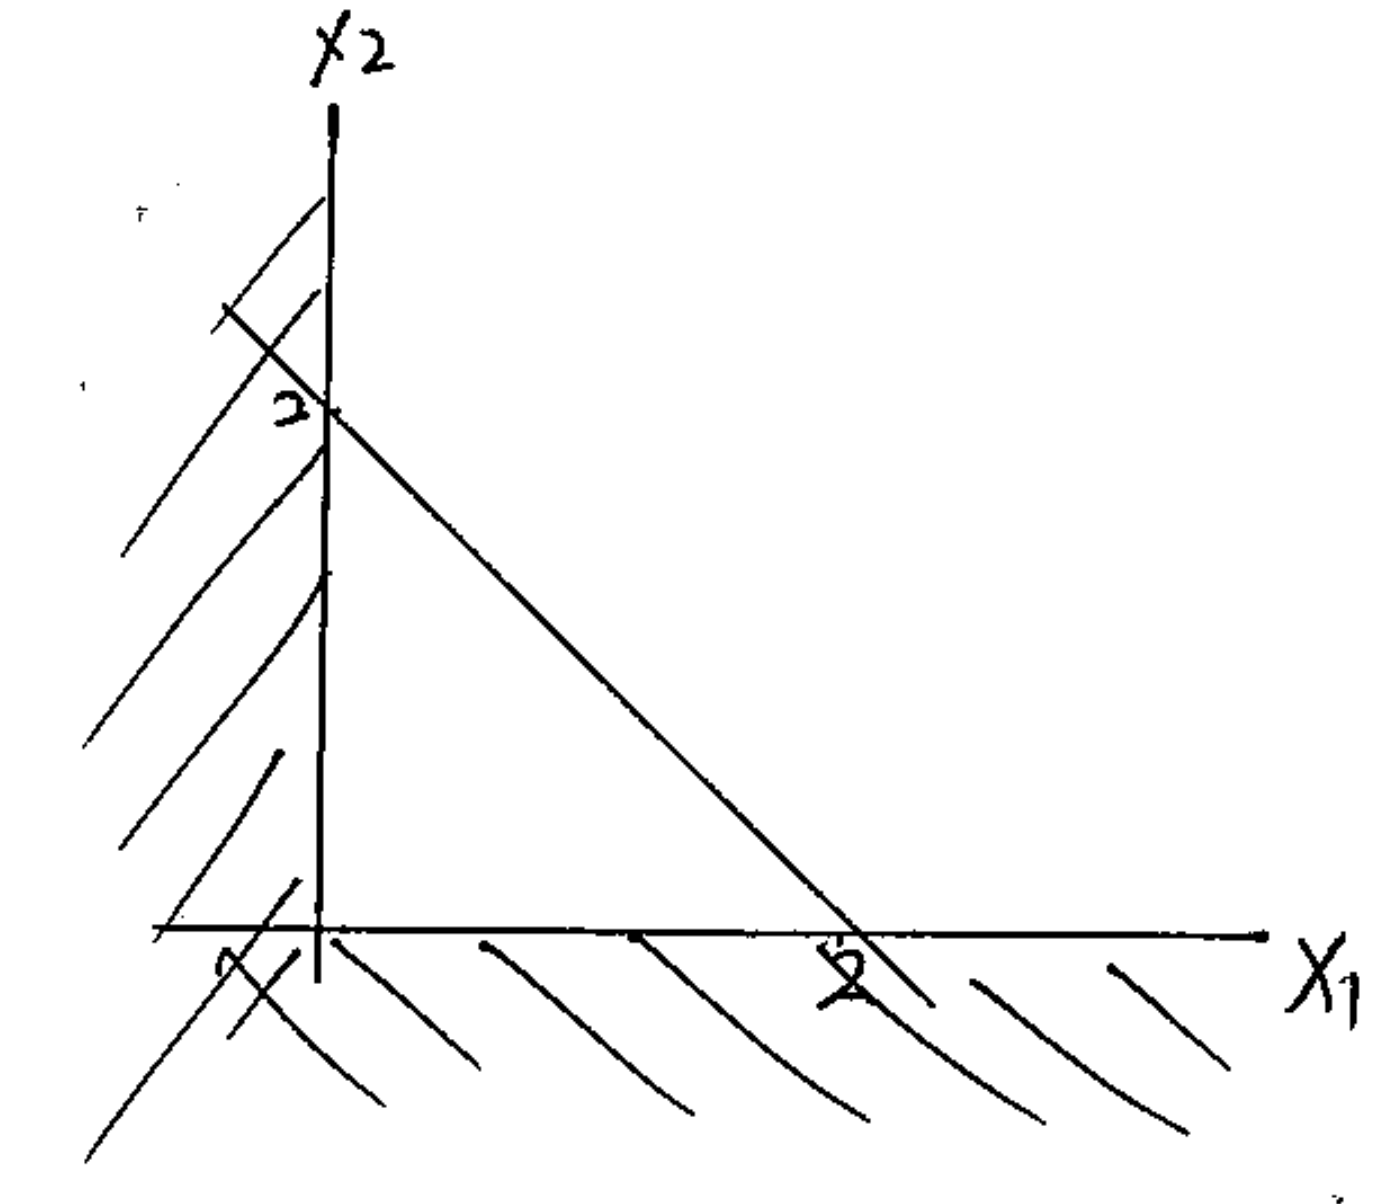
\includegraphics[width=2.1in,height=2.1in]{figures/ch07/figure1012_2.png}
	%\caption{This is an inserted JPG graphic} 
	%\label{fig:graph} 
	\end{figure}
\end{example}








\begin{example}
	Equality constraints force you into lower effective dimension:
	
	\begin{align*}
	A =
	\begin{bmatrix}
	1&1&1
	\end{bmatrix}
	\end{align*}
	\begin{equation*}
	B= 
	\begin{bmatrix}
	1\\
	\end{bmatrix}
	\end{equation*}
	
	\begin{figure}
	\centering
	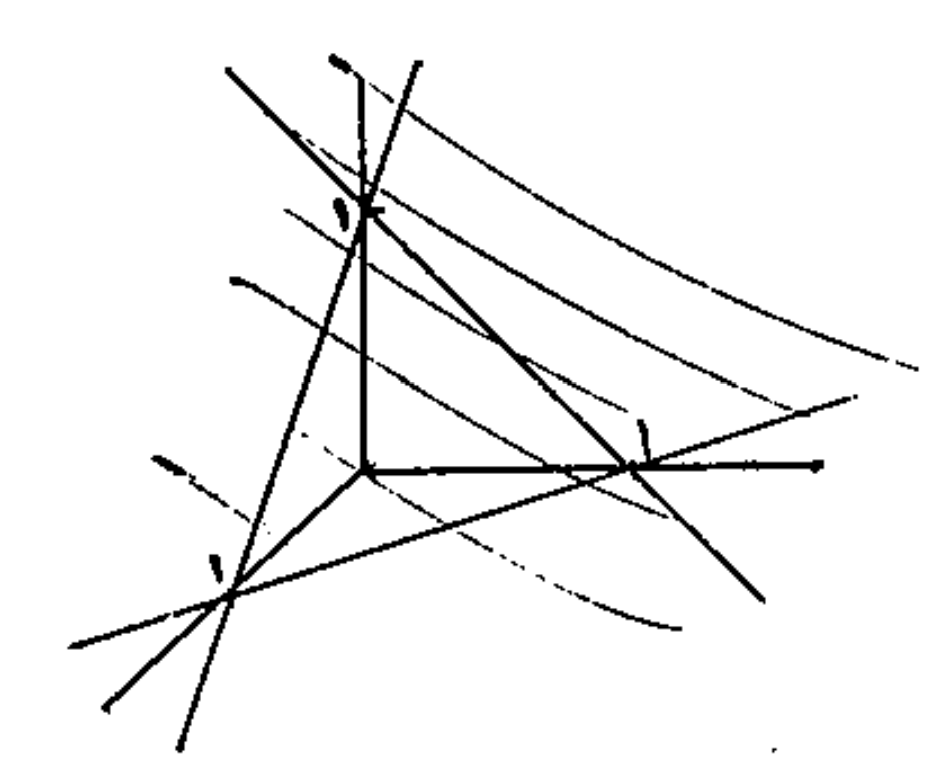
\includegraphics[width=2.1in,height=2.1in]{figures/ch07/figure1012_3.png}
	%\caption{This is an inserted JPG graphic} 
	%\label{fig:graph} 
	\end{figure}
\end{example}

\begin{example}
	\begin{equation*}
	\begin{bmatrix}
	1&1\\
	1&1
	\end{bmatrix}
	\begin{bmatrix}
	x_1\\
	x_2
	\end{bmatrix}=
	\begin{bmatrix}
	1\\
	2
	\end{bmatrix}
	\end{equation*}
	
	\begin{figure}
	\centering
	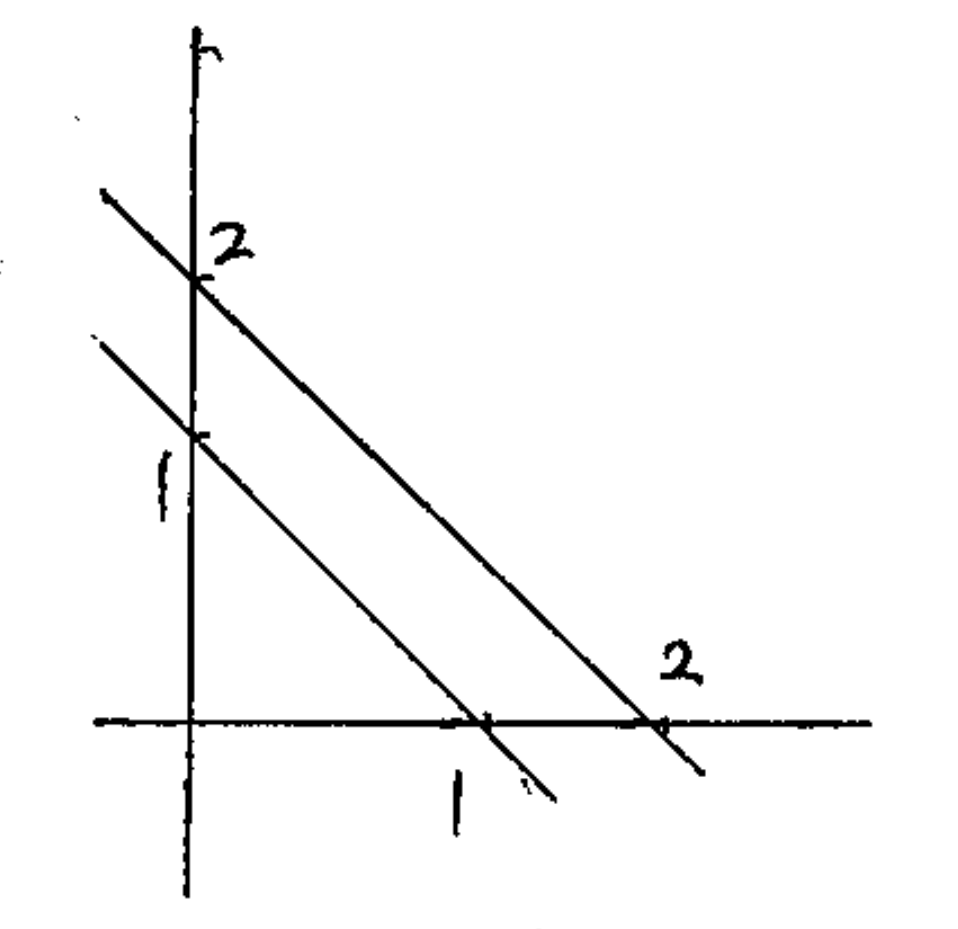
\includegraphics[width=2.1in,height=2.1in]{figures/ch07/figure1012_4.png}
	%\caption{This is an inserted JPG graphic} 
	%\label{fig:graph} 
	\end{figure}
	
	Can also happen with inequalities constraints:
		\begin{align*}
	\begin{bmatrix}
	-1&0\\
	1&0
	\end{bmatrix}
	\begin{bmatrix}
	x_1\\
	x_2
	\end{bmatrix}&\leq
	\begin{bmatrix}
	0\\
	-1
	\end{bmatrix}\\
	S &= \emptyset
	\end{align*}

\end{example}



\begin{example}
	\begin{align*}
	\begin{bmatrix}
	-1 & 0\\
	0 & -1\\
	\frac{1}{2} & -1\\
	1 & 1
	\end{bmatrix}
	\begin{bmatrix}
	x_1\\
	x_2
	\end{bmatrix}
	 &\leq 
	 \begin{bmatrix}
	 0\\
	 0\\
	 1\\
	 3
	 \end{bmatrix}\\
	 \frac{1}{2}x_1 - x_2&\leq 1\\
	 x_2 &\geq -1 + \frac{1}{2}x_1
	\end{align*}
	
	\begin{figure}
	\centering
	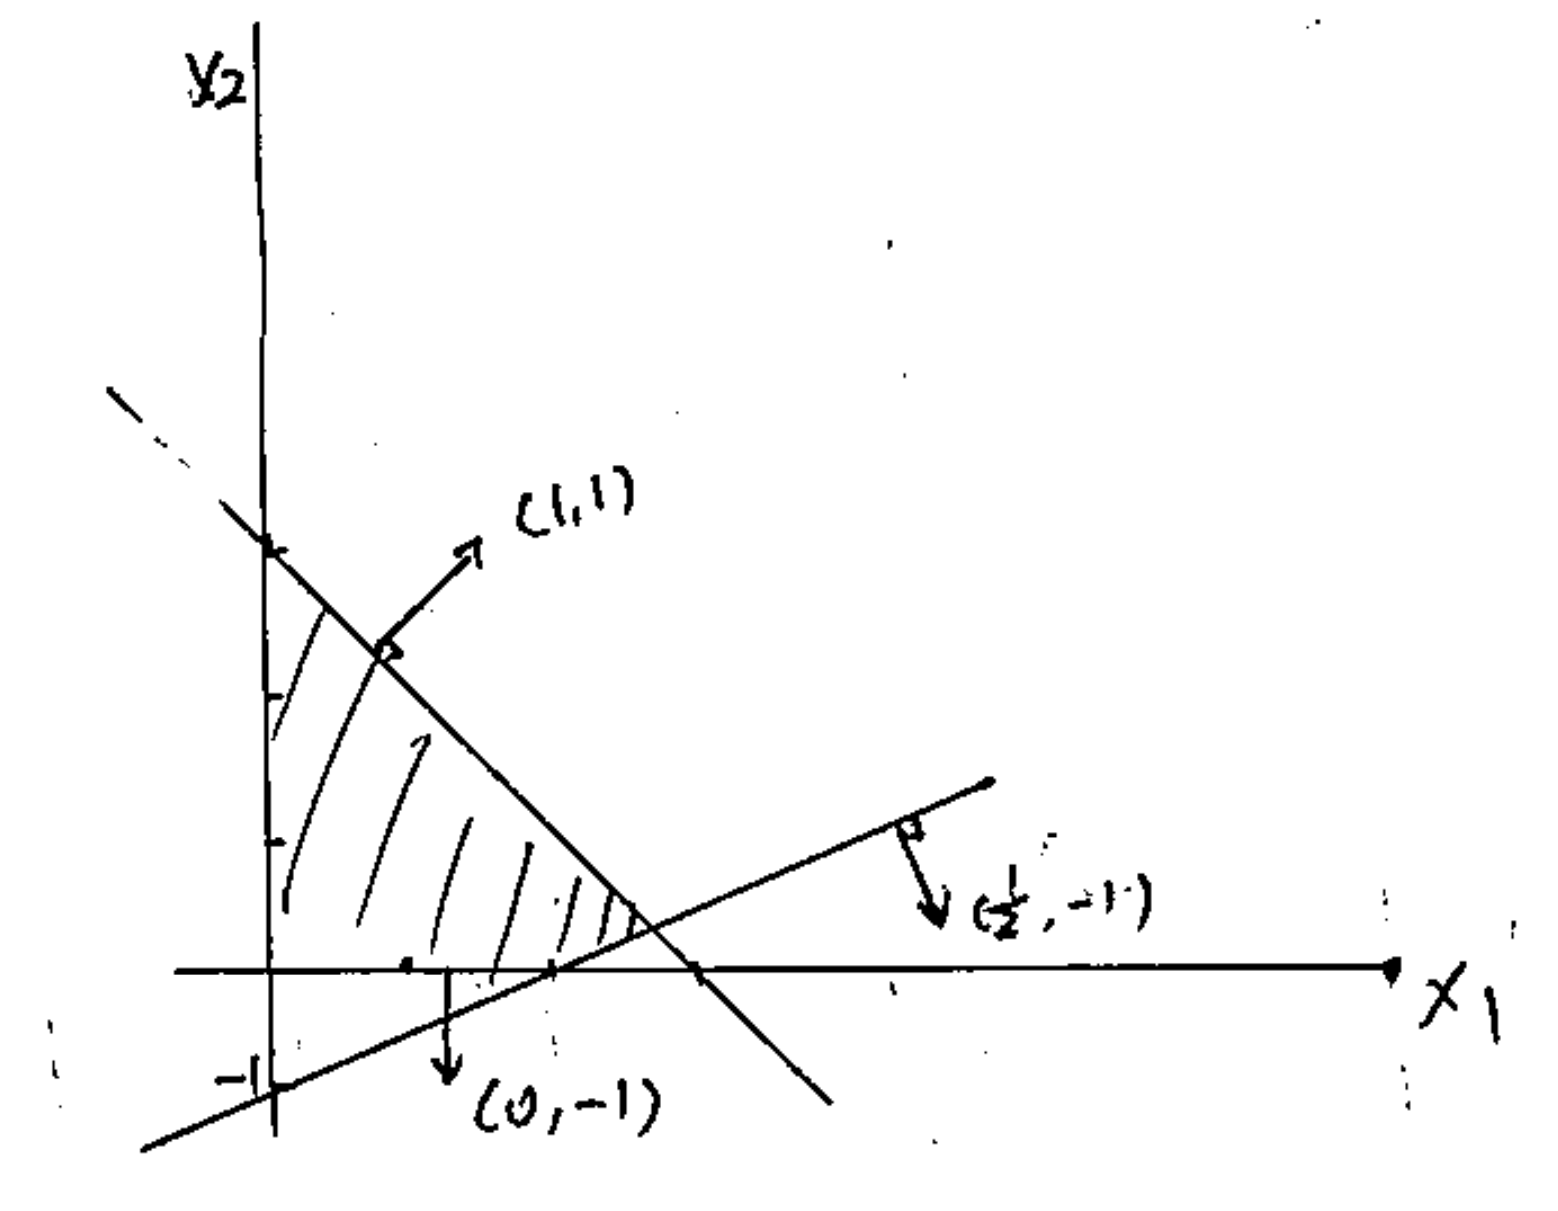
\includegraphics[width=2.1in,height=2.1in]{figures/ch07/figure1012_5.png}
	%\caption{This is an inserted JPG graphic} 
	%\label{fig:graph} 
	\end{figure}
\end{example}





LP: Linear objective \& constraints

\begin{figure}
	\centering
	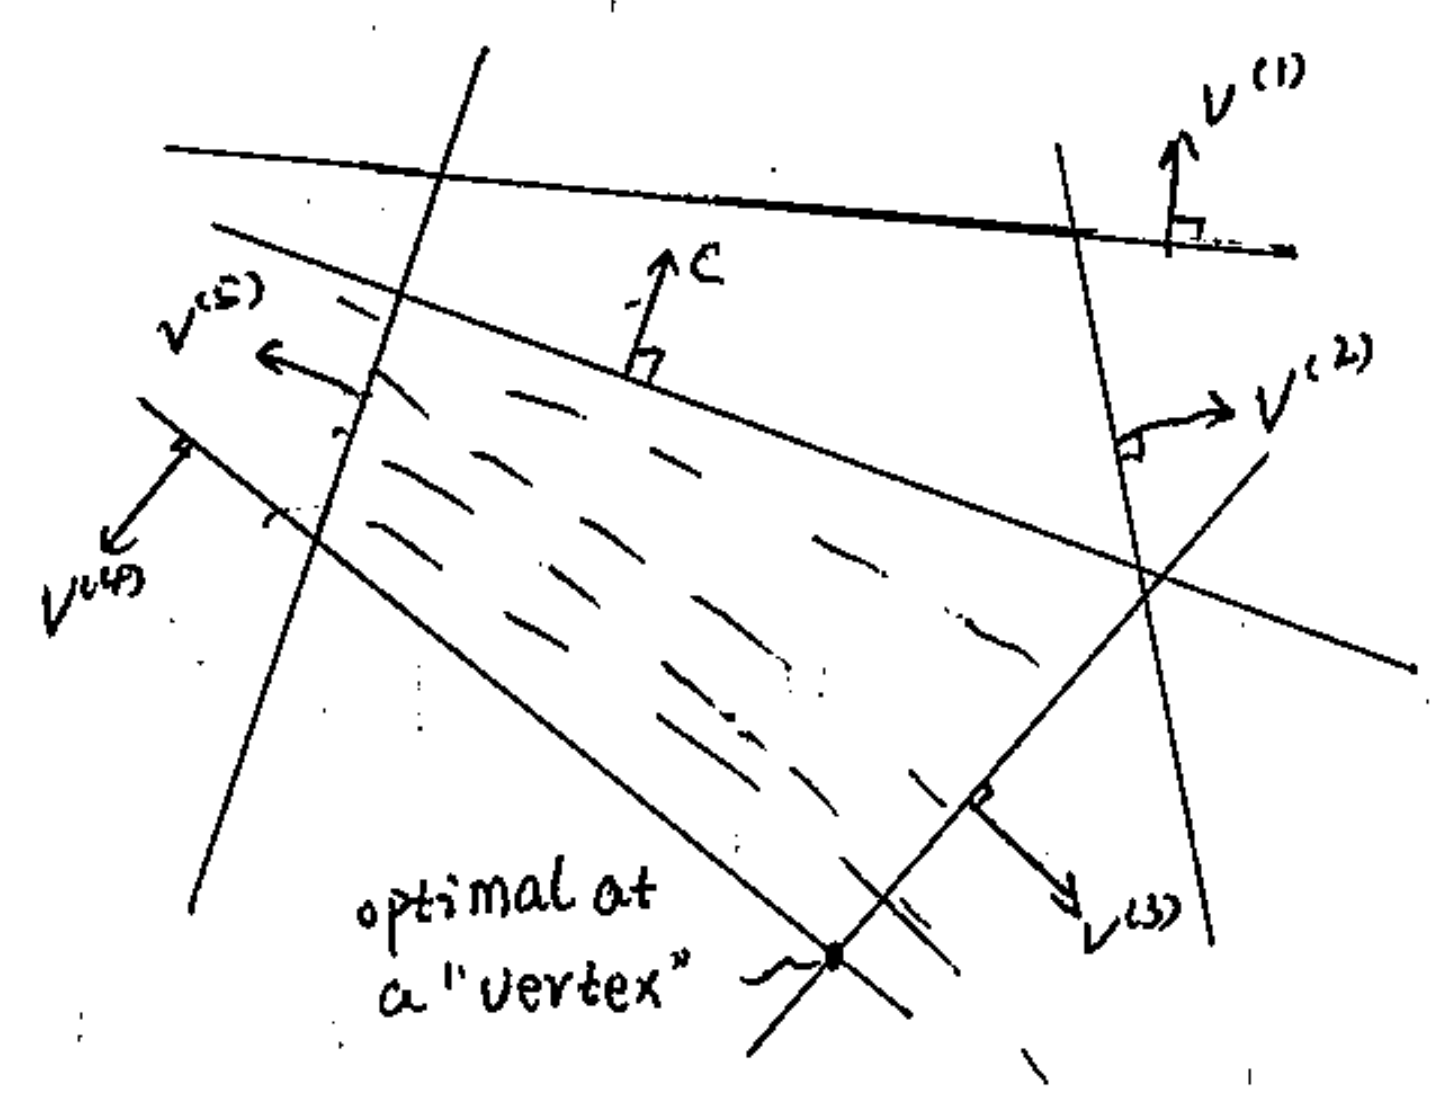
\includegraphics[width=2.1in,height=2.1in]{figures/ch07/figure1012_6.png}
	%\caption{This is an inserted JPG graphic} 
	%\label{fig:graph} 
\end{figure}

\begin{equation*}
S = \{x\in \Re^3 | 
\begin{bmatrix}
1 & 1 & 1
\end{bmatrix}
\begin{bmatrix}
x_1\\
x_2\\
x_3
\end{bmatrix}
 = 1, x_1 \geq 0, x_2\geq 0,x_3\geq 0
 \}
\end{equation*}

\begin{align*}
x^* = arg\,\,\, &min 
\begin{bmatrix}
1&1&1
\end{bmatrix}x\\
&s.t. \,\,\, x\in S\\
x^* = arg\,\,\, &min 
\begin{bmatrix}
1&0&0
\end{bmatrix}x = x_1\\
\end{align*}

\begin{figure}
	\centering
	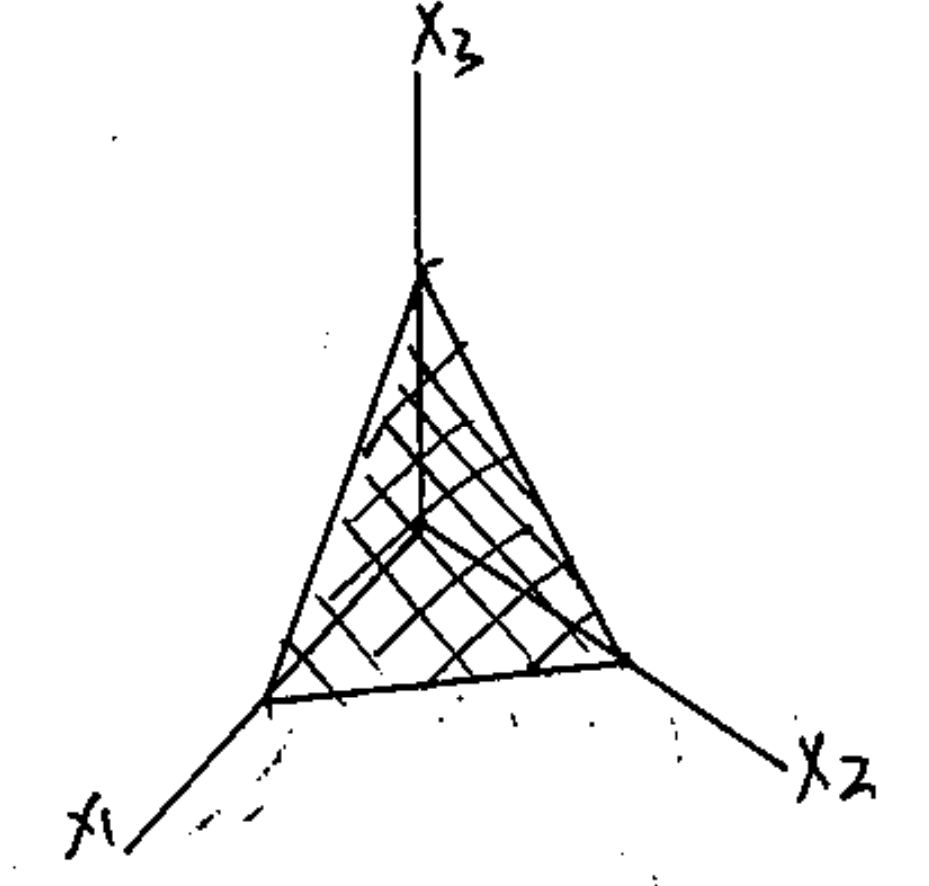
\includegraphics[width=2.1in,height=2.1in]{figures/ch07/figure1012_7.png}
	%\caption{This is an inserted JPG graphic} 
	%\label{fig:graph} 
\end{figure}

So there are various possibilities here for $p^* \& x^* $:

\begin{itemize}
	\item 1) $x^*$ is unique, $p^*$ finite
	
	\item 2) $x^*$ is not unique, $p^*$ finite. 
	
	\item 3) There is no $x^*$:
	
		a) $S = \emptyset$(Feasible set is empty), constraint $p^* = \infty$
	
		b) $S$ is unbounded \& no minimum, constraint $p^* = -\infty$
\end{itemize}


\begin{figure}
	\centering
	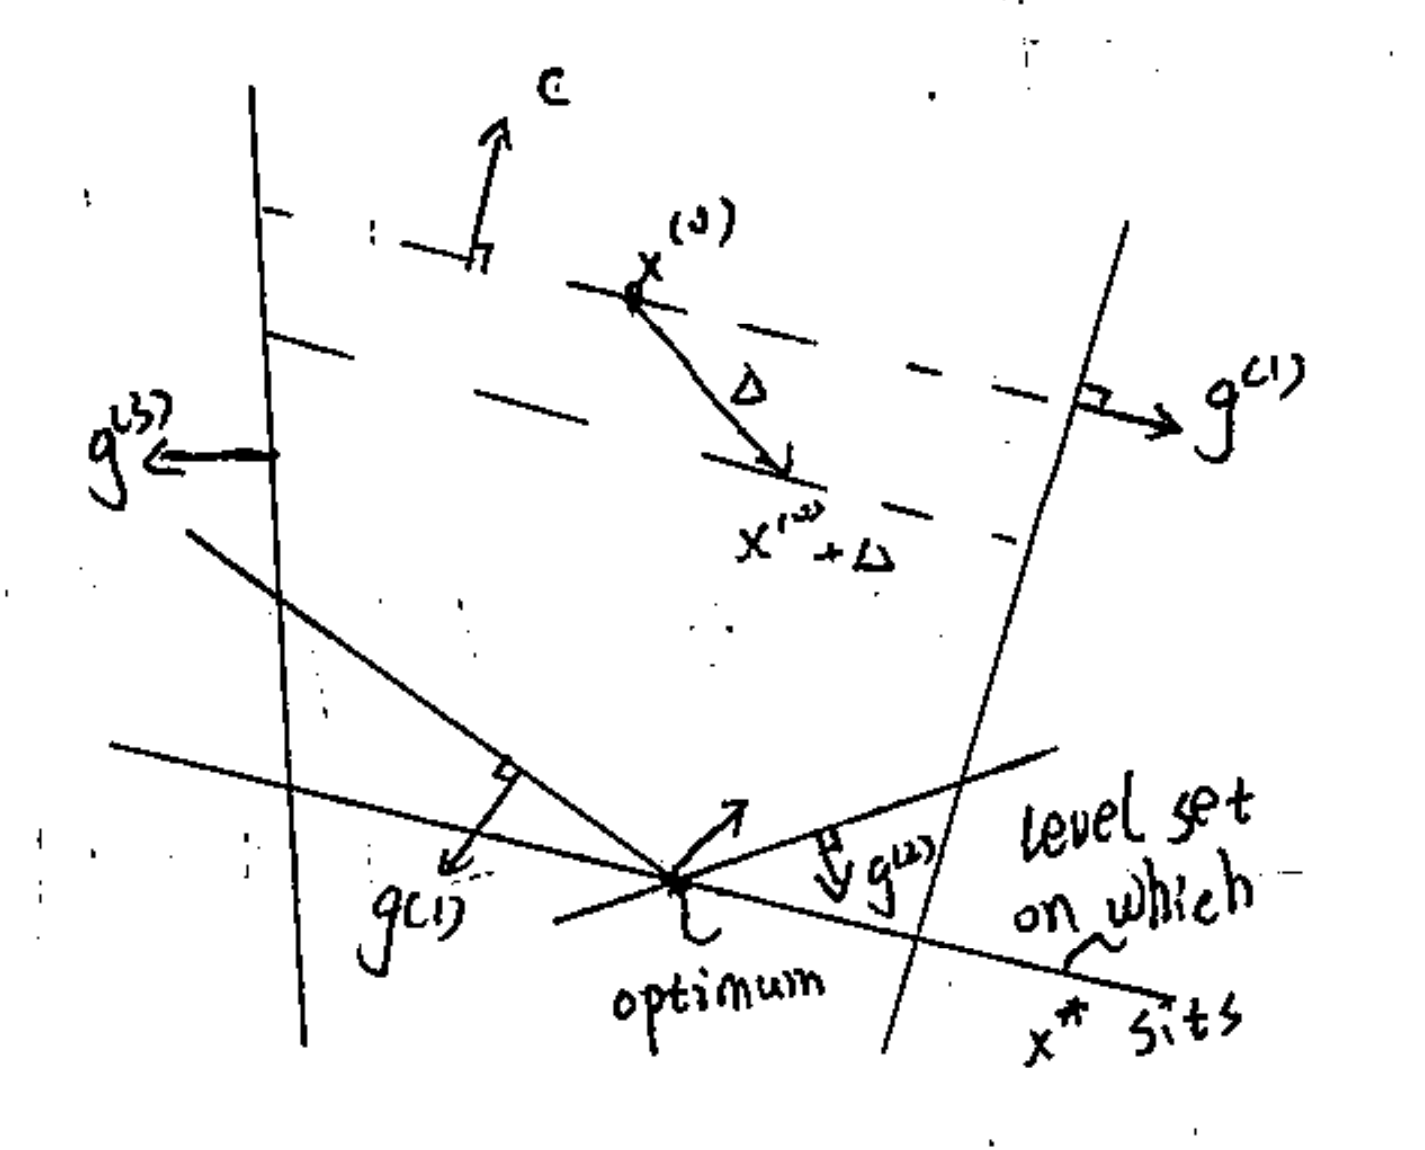
\includegraphics[width=2.1in,height=2.1in]{figures/ch07/figure1012_8.png}
	%\caption{This is an inserted JPG graphic} 
	%\label{fig:graph} 
\end{figure}





"active" constraints are those inequality constraints satisfied with equality. 

Cost decreases if:

\begin{align*}
c^T(x^{(0)} + \bigtriangleup) + d &< c^Tx^{(0)} + d\\
c^T\bigtriangleup &< 0\\
<c, \bigtriangleup> &< 0
\end{align*}


In example constraints 1\&2 are active at optimum.\\

Observation: 

\begin{itemize}
	\item If you are at a vertex(doesn't have to be optimum). 
	
	\item Any "move" that keeps you feasible must be into feasible set $\rightarrow$ opposite vector that define active constraints.
	
	\begin{equation*}
	v - \alpha g^{(1)} - \beta g^{(2)}, \,\,\, \alpha, \beta \geq 0
	\end{equation*}
	
	\item Are these any choices of $\alpha, \beta$ that decrease the cost?
	
	\begin{align*}
	c^T(v - \alpha g^{(1)} - \beta g^{(2)}) + d &\leq c^Tx + d\\
	-\alpha <c, g^{(1)}> - \beta<c, g^{(2)}> &\leq 0
	\end{align*}
\end{itemize}

If:

1) $<c, g^{(1)}> < 0$

2) $<c, g^{(2)}> < 0$

no more into feasible set will decrease the cost.\\ 

Condition for optimality:\\

A feasible vertex $v$: $v\in\{x|Gx \leq h \}$ is an optimal solution to LP with cost $F_0(x) = c^Tx + d$ if $c^Tg^{(i)} < 0$, $\forall i\in$ active set.\\

\begin{figure}
	\centering
	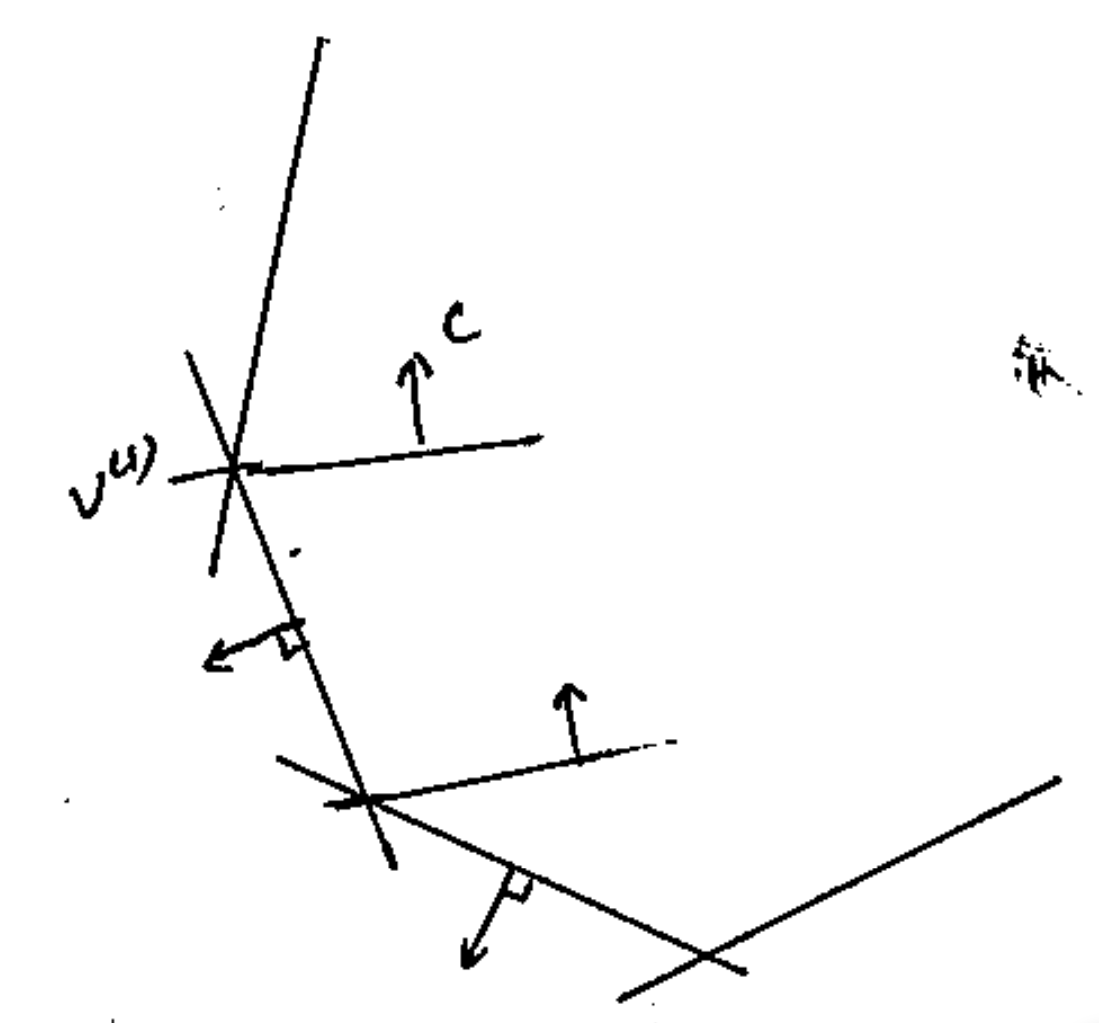
\includegraphics[width=2.1in,height=2.1in]{figures/ch07/figure1012_9.png}
	%\caption{This is an inserted JPG graphic} 
	%\label{fig:graph} 
\end{figure}


Simplex algorithm:

\begin{itemize}
	\item 1) Start ar feasible vertex;
	
	\item 2) Identify direct of cost decrease along an edge;
	
	\item 3) Move on that direction until any further more would violate a previously inactive constraints.
	
	\item 4) Stop + add that new constraint(s) to active set.
	
	\item 5) Repeat
\end{itemize}



%Above are notes for Oct 12

%Below are notes for Oct14



\begin{equation*}
\{x|Gx\leq h \}
\end{equation*}


\begin{figure}
	\centering
	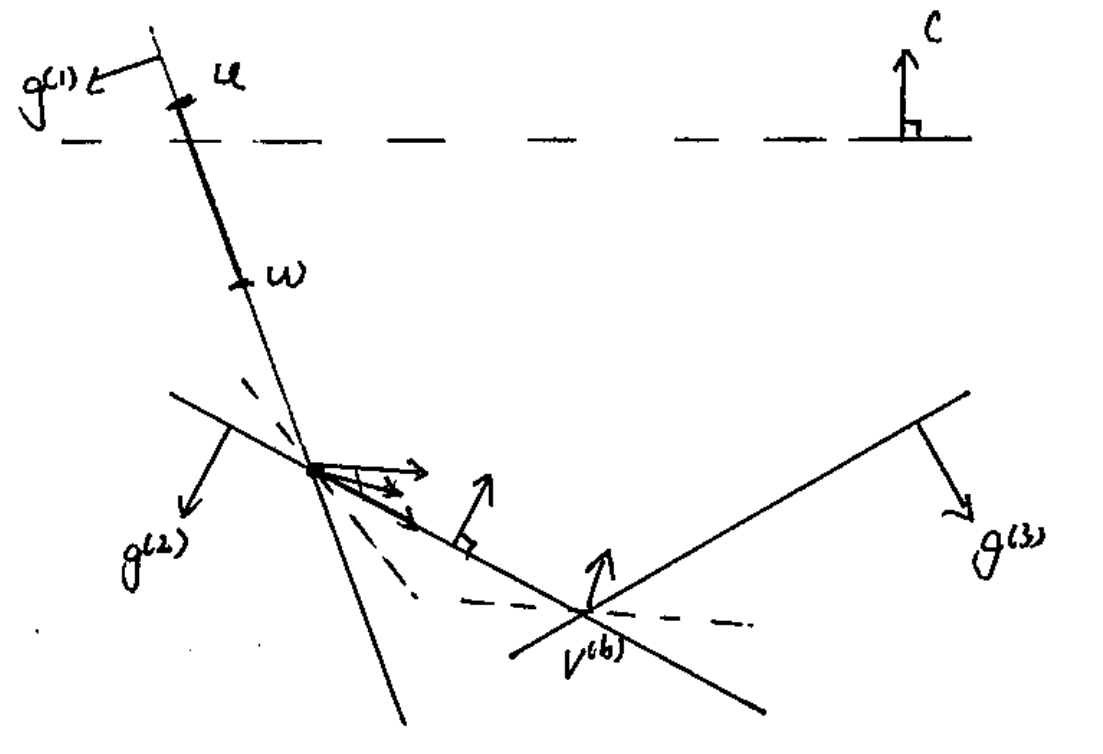
\includegraphics[width=2.1in,height=2.1in]{figures/ch07/figure1016_1.png}
	%\caption{This is an inserted JPG graphic} 
	%\label{fig:graph} 
\end{figure}


If $x =v^{(a)}$, constraints, constraints 1\&2 active, 3 is inactive.

\begin{align*}
<g^{(1)}, v^{(a)}> &= h_1\\
<g^{(2)}, v^{(a)}> &= h_2\\
<g^{(3)}, v^{(a)}> &< h_3
\end{align*}

At $x = v^{(b)}$, constraints 2\&3 active, 1 is inactive.\\

1) Define a vertex $v$:

\begin{itemize}
	\item a) $v\in S$ is a vertex if cannot express $v = \lambda u +(1-\lambda)w$, $u, w\in S$, $\lambda \in [0,1]$
	
	\item b) There exists a cost vector $c\in \Re^n$ s.t. $v$ is unique solution to an LP with cost vector $c$.
	
	\item c) Algebraic characterization of vertices in terms of $A, b, G, h$. $S = \{x|Ax \leq b, Gx\leq h \}$
\end{itemize}



2) Define / Find directions along edges of polyhedron that keep you in the feasible set.

3) How far can you go in direction that decrease cost until "leave" feasible set?

\begin{align*}
min \,\,\, &c^Tx+d\\
s.t. \,\,\, &Ax = b\\
&Gx\leq h
\end{align*}

$x\in \Re^n, c\in \Re^n, d\in \Re, A\in \Re^{q\times n}, b\in \Re^q, G\in \Re^{m\times n}, h\in \Re^m$.

Inequalities:

\begin{align*}
min \,\,\, &c^Tx+d\\
s.t. \,\,\, &Gx\leq h\\
\end{align*}

"Standard Form":

\begin{align*}
min \,\,\, &c^Tx+d\\
s.t. \,\,\, &Ax = b\\
&x\geq 0
\end{align*}

To get to inequality:

\begin{equation*}
Ax = b \Leftrightarrow Ax\geq b, Ax\leq b
\end{equation*}

\begin{align*}
min\,\,\, &c^Tx +d\\
s.t. &\begin{bmatrix}
G\\
A\\
-A
\end{bmatrix} x\leq
\begin{bmatrix}
h\\
b\\
-b
\end{bmatrix}
\end{align*}

Standard Form:

\begin{align*}
min \,\,\, &c^Tx+d\\
s.t. \,\,\, &Gx\leq h\\
&Ax = b
\end{align*}

is equivalent to:

\begin{align*}
min \,\,\, &c^Tx+d\\
s.t. \,\,\, &Gx + s = h\\
&Ax = b\\
&s\geq 0
\end{align*}

is also equivalent to:

\begin{align*}
min \,\,\, &c^T(x^{+} - x^{-})+d\\
s.t. \,\,\, &G(x^{+} - x^{-}) + s = h\\
&A(x^{+} - x^{-}) = b\\
&s\geq 0\\
&x^{+}\geq 0\\
&x^{-}\geq 0
\end{align*}

can come to:

\begin{align*}
min_{x^{+},x^{-},s} &\begin{bmatrix}
c^T - c^T & 0
\end{bmatrix}
\begin{bmatrix}
x^{+}\\
x^{-}\\
s
\end{bmatrix}+d\\
&\begin{bmatrix}
A-A & 0
\end{bmatrix}
\begin{bmatrix}
x^{+}\\
x^{-}\\
s
\end{bmatrix}=b\\
&\begin{bmatrix}
G-G & I
\end{bmatrix}
\begin{bmatrix}
x^{+}\\
x^{-}\\
s
\end{bmatrix}=h\\
&x^{+}\geq 0, x^{-}\geq 0, s\geq 0
\end{align*}




\begin{example}
	\begin{align*}
	&min \Vert Ax - b\Vert_{\infty}\\
	&s.t. Gx \leq h\\
	&\Vert u\Vert_{\infty} = max_{i\in [n]}|u_i|
	\end{align*}
	Introduce helper variable $t$:
	
	\begin{figure}
	\centering
	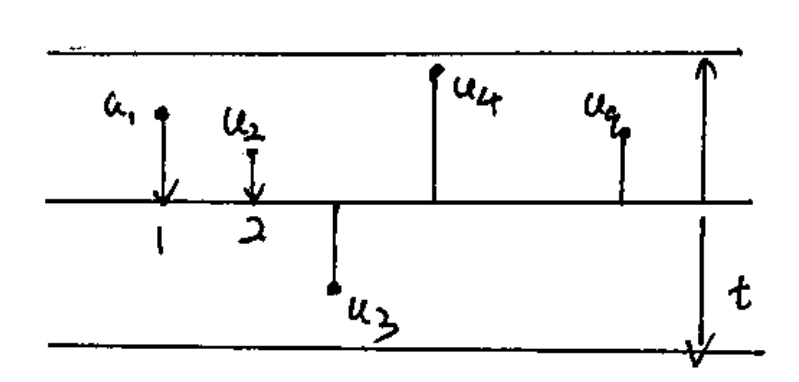
\includegraphics[width=2.1in,height=2.1in]{figures/ch07/figure1016_2.png}
	%\caption{This is an inserted JPG graphic} 
	%\label{fig:graph} 
	\end{figure}
	
	
	\begin{align*}
	min_{x,t} &t\\
	s.t. &Ax - b\leq t\textbf{1}\\
	&Ax - b\leq (-t)\textbf{1}\\
	&Gx \leq h
	\end{align*}
\end{example}


\begin{example}
	\begin{figure}
	\centering
	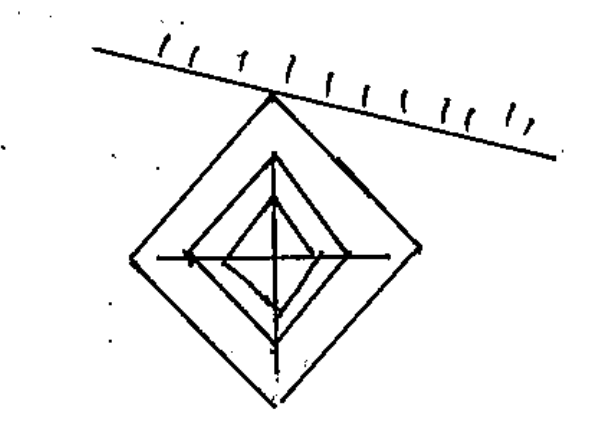
\includegraphics[width=2.1in,height=2.1in]{figures/ch07/figure1016_3.png}
	%\caption{This is an inserted JPG graphic} 
	%\label{fig:graph} 
	\end{figure}
	
	\begin{align*}
	min_x &||Ax - b||_1, \,\,\,\,\, A\in \Re^{q\times n}\\
	s.t. &Gx\leq h
	\end{align*}
	
	\begin{equation*}
	||u||_1 = \sum^q_{i=1} |u_i|
	\end{equation*}
	
	Helper vector $t\in \Re^q$.
	
	\begin{align*}
	min_{x,t} &\sum^q_{i=1}t_i\\
	s.t. \,\,\,\,\,&Gx \leq h\\
	&Ax -b \leq t\\
	&Ax -b \geq -t
	\end{align*}
	
	\begin{figure}
	\centering
	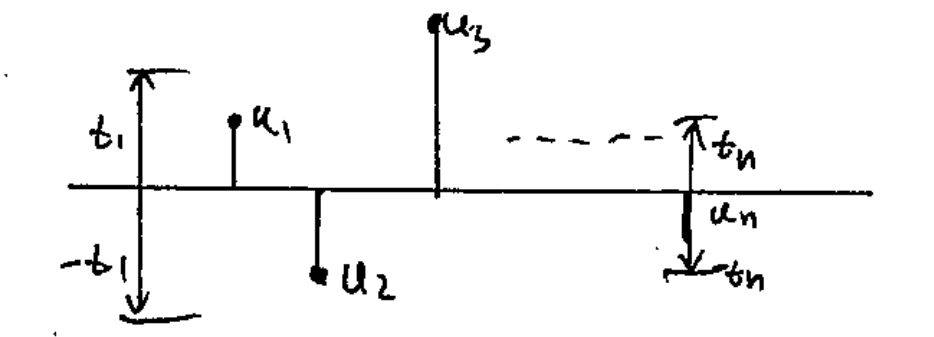
\includegraphics[width=2.1in,height=2.1in]{figures/ch07/figure1016_4.png}
	%\caption{This is an inserted JPG graphic} 
	%\label{fig:graph} 
	\end{figure}
\end{example}

\begin{example}
	\begin{align*}
	min \,\,\, max_{i\in [q]} &(c^{(i)^T}x + d_i)\\
	s.t. &Gx\leq h
	\end{align*}
	
	\begin{align*}
	min_{x, t\in \Re} &t\\
	s.t. &(c^{(i)^T}x + d_i)\leq t,\,\,\,\,\, \forall i\in [q]\\
	&Gx\leq h
	\end{align*}
	
	\begin{figure}
	\centering
	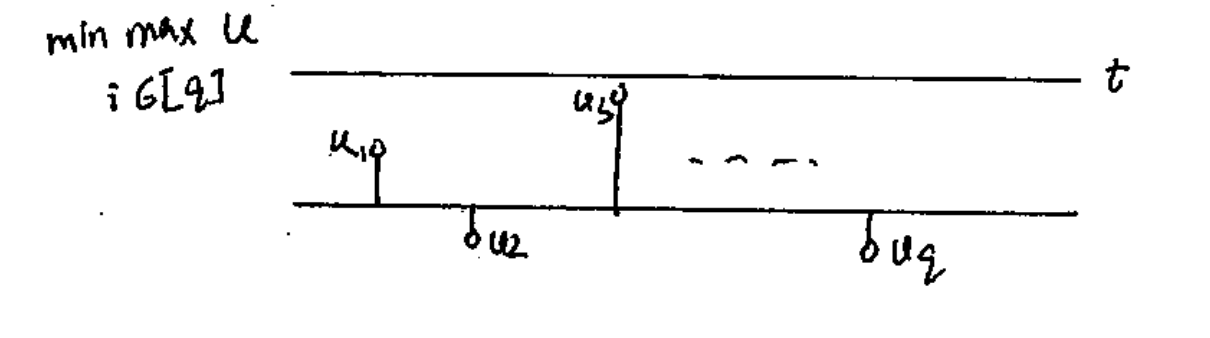
\includegraphics[width=2.1in,height=2.1in]{figures/ch07/figure1016_5.png}
	%\caption{This is an inserted JPG graphic} 
	%\label{fig:graph} 
	\end{figure}
\end{example}



\begin{example}
	Finding the largest $l_2$ ball that fits in a polyhedron $p = \{x| Gx\leq h \}$
	
	\begin{figure}
	\centering
	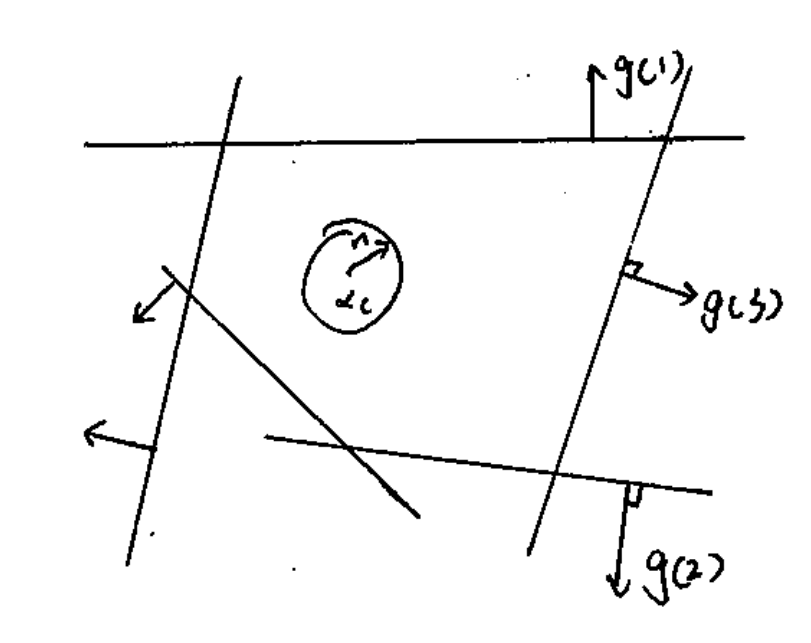
\includegraphics[width=2.1in,height=2.1in]{figures/ch07/figure1016_6.png}
	%\caption{This is an inserted JPG graphic} 
	%\label{fig:graph} 
	\end{figure}
\end{example}

A sphere is fully parameterized by :
\begin{itemize}
	\item Its center $x_c$
	
	\item Its radius $r$
\end{itemize}

A sphere fits in $p$ if:$x_c + u \in p$, $\forall u \,\,\, s.t. ||u||_2\leq r$


\begin{itemize}
	\item $x_c+u \in p$ means that $g^{(i)^T}(x_c + u) \leq h_i,\,\,\, \forall i\in [q]$ \& all $u$ $s.t. ||u||_2\leq r$.
	
	\item Looking at constraints $i$ by itself: $g^{({i})^T}x_c + g^{({i})^T}u \leq h_i$. 
	
	As for $g^{({i})^T}u$, for $||u||_2>r$, what direction should $u$ point in to make left hand side as large as possible?
	
	Set $u=\frac{g^{(1)}}{||g^{(1)}||}r$ 
\end{itemize}

Upshot: if following is satisfied:

\begin{equation*}
g^{(1)^T}[x_c + \frac{g^{(1)}}{||g^{(1)}||_2}r] \leq h_i
\end{equation*}

Then constraint $i$ is satidfied for all $u$ that are of length $r$.



\begin{align*}
max_{x, r} &r\,\,\,(or\,\,\,min -r)\\
s.t. &g^{(1)^T}x_c + ||g^{(1)}||_r\leq h_i\,\,\,\,\, i\in [q]
\end{align*}

$\rightarrow(x_c, r)\in \Re^{n+1}$

$\rightarrow$ Transformed some quadratic-like problem into an LP.\\


Quadratic program(QP)

\begin{align*}
p^* = min_{x\in \Re^n} &\frac{1}{2}x^THx + c^Tx + d\\
s.t. \,\,\, &Ax = b\\
&Gx \leq h
\end{align*}

\begin{figure}
	\centering
	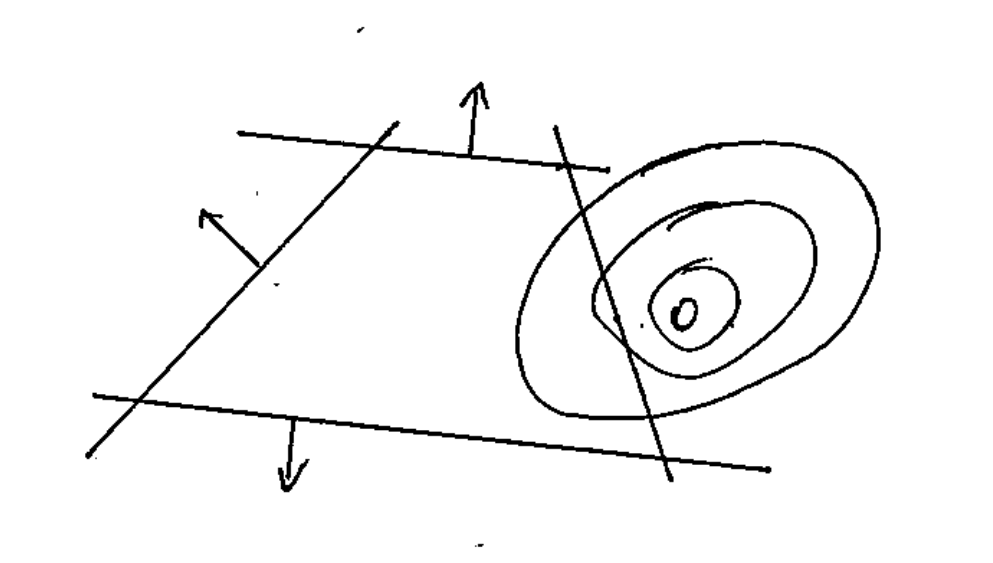
\includegraphics[width=2.1in,height=2.1in]{figures/ch07/figure1016_7.png}
	%\caption{This is an inserted JPG graphic} 
	%\label{fig:graph} 
\end{figure}
%Above are notes for Oct14


\section{10.16}

%Below are notes for Oct16

\begin{align*}
p^* = min_{x\in \Re^n}\,\,\,\,\, &\frac{1}{2}x^THx + c^Tx + d\\
 s.t.\,\,\,\,\, &Ax = b\\
 &Gx\leq h
\end{align*}


\begin{figure}
	\centering
	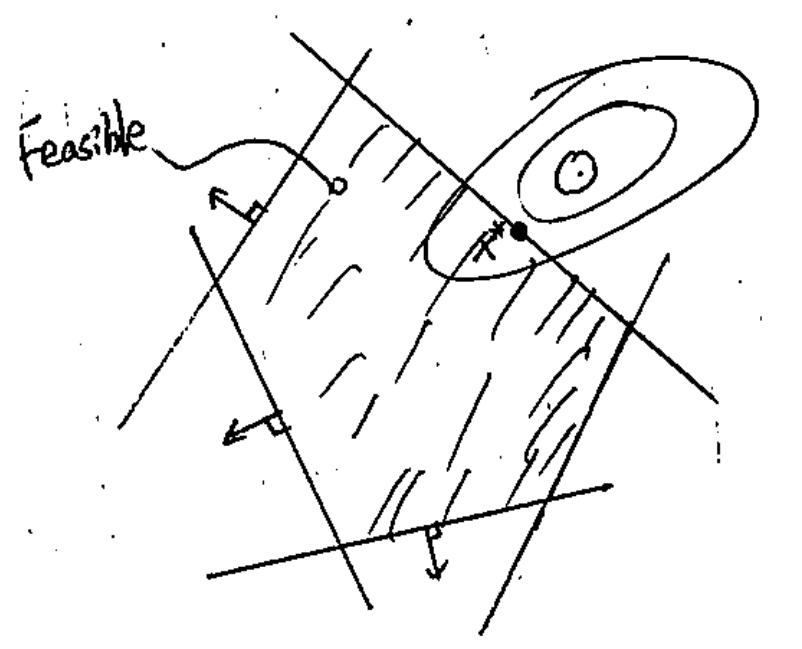
\includegraphics[width=2.1in,height=2.1in]{figures/ch07/figure1016_a.png}
	%\caption{This is an inserted JPG graphic} 
	%\label{fig:graph} 
\end{figure}

\subsection{Least squares}
\begin{align*}
||Ax - y||_2^2 &= (Ax - y)^T(Ax - y)\\
&= x^TA^TAx - 2y^TAx + y^Ty\\
&= \frac{1}{2}x^T(2A^TA)x - 2y^TAx + ||y||_2^2
\end{align*}

Note: Cannot always manipulate objective of a QP into form of objective of a LS problem.\\

\subsection{Equality constrained QPs}

\begin{align*}
p^* = min_{x\in \Re^n}\,\,\,\,\, &\frac{1}{2}x^THx + c^Tx + d\\
s.t.\,\,\,\,\, &Ax = b
\end{align*}


\begin{figure}
	\centering
	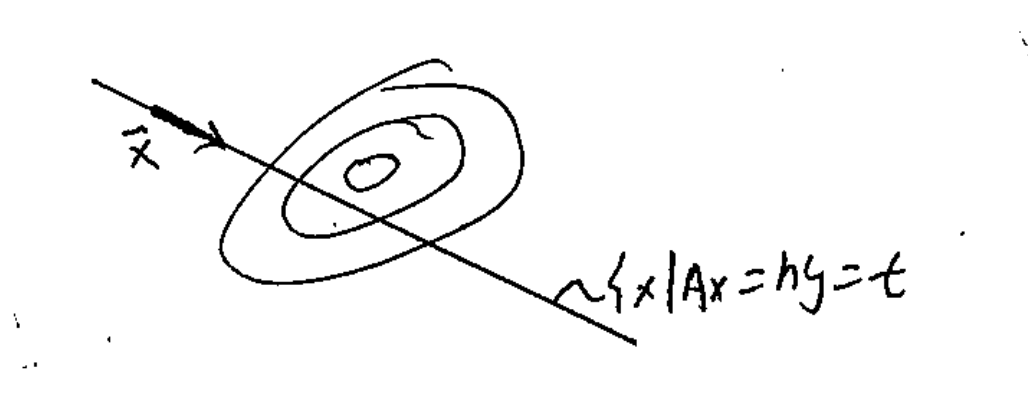
\includegraphics[width=2.1in,height=2.1in]{figures/ch07/figure1016_b.png}
	%\caption{This is an inserted JPG graphic} 
	%\label{fig:graph} 
\end{figure}

\begin{equation*}
\mathcal{A} =\{x | x = \bar{x} + \xi,\,\,\, \text{where } \xi \in N(A) \}
\end{equation*}

Let N be a basis for $N(A)$, can express $\xi \in N(A)$ as $\xi = Nz$ where $z\in \Re^k$, $k =dim(N(A)) \leq n$


Substitute this expression for any feasible $x$ into objective $F_0(\cdot)$


\begin{align*}
F_0(x) &= F_0(\bar{x} + \xi) = F_)(\bar{x} + Nz)\\
&= \frac{1}{2}(\bar{x} + Nz)^TH(\bar{x}+Nz) + c^T(\bar{x} + Nz) + d\\
&= \frac{1}{2}z^T[N^THN]z + [c^TN + \bar{x}^THN]z + [\frac{1}{2}\bar{x}^TH\bar{x} + c^Tx + d] \\
\end{align*}

\begin{equation*}
p^* = min_{z\in \Re^k}\,\,\,\,\, \frac{1}{2}z^T\tilde{H}z + \tilde{c^T}z + \tilde{d}
\end{equation*}

$\rightarrow$ lower-dimensional optimization problem $k =dim(N(A)) \leq n $

$\rightarrow$ still a QP, but an unconstrained QP.



\begin{example}{Markowitz Partfolio optimization}
	"Mean/variance" analysis
	
	\begin{itemize}
		\item Minimize amount of variance in returns for a fixed level of (expected) returns
		
		\item Harry Markowitz(1990 Nobel Prize)
	\end{itemize}
	
	\textbf{Model}: There are n stock, single investment period\\
	
	\textbf{Task}:
	
	\begin{itemize}
		\item Design an investment strategy $p\in \Re^n$
		
		\item $p_i = $ amount/proportion of wealth invested in stock $i$
		
		\item $\sum^n_{i=1}p_i = 1$, "all-in" invest all your money
		
		\item $p_i \geq 0$, "long" positions(no "short time")
		
		\item Wealth normalized to 1
	\end{itemize} 
	
	\textbf{Returns}:
	
	\begin{itemize}
		\item $x\in \Re^n$
		
		\item $x_i$ = return on $i^th$ stock in period if must 1RMB in stock: get $x_i$RMB back.
	\end{itemize} 
	
	
	\textbf{Probabilistic model on returns}:
	
	\begin{itemize}
		\item Expected returns: $\bar{x_i} = \mathbb{E}[x_i]$(known)
		
		\item Your return (random) is $\sum^n_{i=1}p_ix_i = p^Tx$
		
		\item Your expected value $\mathbb{E}[\sum^n_{i=1}p_ix_i] = \sum^n_{i=1}p_i\mathbb{E}[x_i] = \sum^n_{i=1}p_i\bar{x_i} = p^T\bar{x}$
		
		\item variance in returns:
		
		\begin{align*}
		var(p^Tx) &=\mathbb{E}[(p^Tx - p^T\bar{x})^2]\\
		&= \mathbb{E}[(p^T(x - x^T))^2]\\
		&= \mathbb{E}[p^T(x - \bar{x})(x - \bar{x})^Tp]\\
		&= p^T\mathbb{E}[(x - \bar{x})(x - \bar{x})^T]p\\
		&= p^T\Sigma p
		\end{align*}
	\end{itemize}
	
	
	
	
	
	
	
	
	

	
	Given mean returns $\bar{x}$ and covariance matrix of returns $\Sigma \in \Re^{n\times n}$. Design $p$ to minimize "risk" subject to same minimal returns.:
	
	\begin{align*}
	min_{p\in \Re^n}\,\,\,\,\, &p^T\Sigma p\\
	s.t. \,\,\,\,\,&p^T\bar{x}\geq r_{min}\\
	&\textbf{1}^Tp = 1\\
	&p\geq 0
	\end{align*}
\end{example}




\begin{align*}
p^* = min_{x\in \Re^n}\,\,\,\,\, &\frac{1}{2}x^THx + x^Tx + d\\
s.t.\,\,\,\,\, &Ax = b\\
&Gx\leq h
\end{align*}

Discuss geometry of objective

Discuss geometry of feasible set

1) w.l.o.g assume $H\in S^n$, 

\begin{align*}
x^THx &=\frac{1}{2}[x^THx + x^TH^Tx]\\
 &= \frac{1}{2}x^T(H+H^T)x
\end{align*}

Hence always consider $H$ symmetric.\\



\subsection{Symmetric matrices}

1) Eigenvalues: purely real eigenvalues (can sort)

2) Eigenvectors: can always be chosen $\perp$ and can always diagonalize

\begin{equation*}
H = \mathcal{U}\Lambda \mathbb{U}^T  = \sum^n_{i=1}\lambda_iu^{(i)}u^{(i)^T}
\end{equation*}

For 3 cases:

\begin{equation*}
F_0(x) = \frac{1}{2}x^THx + c^Tx + d
\end{equation*}

\begin{itemize}
	\item A) $H\in S^n$ but not PSD
	
	\begin{equation*}
	H = 
	\begin{bmatrix}
	1&0\\
	0&-2
	\end{bmatrix}
	\end{equation*}
	
	\item B) $H\in S^n_+$ but not PD
	\begin{equation*}
	H = 
	\begin{bmatrix}
	1&0\\
	0&0
	\end{bmatrix}
	\end{equation*}
	
	\item C) $H\in S^n_{++}$
	\begin{equation*}
	H = \begin{bmatrix}
	1&0\\
	0&2
	\end{bmatrix}
	\end{equation*}
\end{itemize}



\begin{itemize}
	\item Plot 1: $F_0(x) =\frac{1}{2}x^THx$
	
	\item Plot 2: $F_0(x) =\frac{1}{2}x^THx + [0.5\,\,\, 0.5]x$
	
	\item Plot 3: $F_0(x) =\frac{1}{2}x^THx + [0.5\,\,\, 0]x$
\end{itemize}




MATLAB Graphs may be included later.\\

Case A: 

$H\in S^n$ but $H\notin S^n_+$. (Symmetric not PSD)

There must be an eigenvalue/vector pair $(\lambda, u)$ s.t. $\lambda < 0$.

Set $x_{\alpha} = \alpha u$ for some $\alpha \in \Re$

\begin{align*}
F_0(\alpha u) &= \frac{1}{2}(\alpha u)^TH(\alpha u) + c^T(\alpha u) + d\\
&= \frac{{\alpha}^2}{2} u^T[\sum^n_{i=1}\lambda_i u^{(i)} u^{(i)^T}]u + \alpha c^Tu + d\\
&= \frac{{\alpha}^2}{2}\lambda + \alpha <c,u> + d\\
&= -\frac{{\alpha}^2}{2}|\lambda| + \alpha<c,u> + d\\
&= F(\alpha u)
\end{align*}


Case B: 

$H\in S_+^n$ but $H\notin S^n_{++}$ (PSD not PD)

$\rightarrow$ at least 1 zero eigenvalue.\\

$c \notin R(H)$

$\rightarrow$ There is a complement of $c$ in $R(H)^{\perp} = N(H^T) = N(H)$ and can move in that direction without changing $2^{nd}$ order term while driving $1^{st} $ order term to $\infty$.

$\rightarrow$ Let $c_{||} = \prod_{R(H)}(c)$, $c_{\perp} = \prod_{N(H)}(c)$

$\rightarrow$ $c = c_{||} + c_{\perp}$ orthogonal decomposition lemma(unique decomposition)

$\rightarrow$ Let $x_{\alpha} =-\alpha c_{\perp}$ where $\alpha \in \Re^+$

\begin{align*}
F_0(x_{\alpha}) &=\frac{{\alpha}^2}{2}c_{\perp}^THc_{\perp} + c^T(-\alpha c_{\perp}) + d\\
&= 0 - \alpha(c_{||} + c_{\perp})^Tc_{\perp} + d\\
&= -\alpha(c_{||}^Tc_{\perp} + c_{\perp}^Tc_{\perp}) + d\\
&= -\alpha||c_{\perp}||^2_2 + d
\end{align*}

\begin{itemize}
	\item Case A: $H\notin S^n_+$, $p^* = -\infty$
	
	\item Case B: $H\in S^n_+$ but not $S^n_{++}$, $c\in R(H)$
	
	\item Case C: $H\in S^n_{++}$
\end{itemize}

%Above are notes for Oct16



%Nelow are notes for Oct21


\section{Geometry of Objective}

\begin{equation*}
p^* = min_{x\in \Re^n}\frac{1}{2}x^THx + c^Tx + d
\end{equation*}

If either (A) $H \notin S^n_+$ then

or (B) - (i): $H\in S^n_+$ but $H\in S^n_{++}$ and $C\notin R(H)$

It comes to $p^* = -\infty$\\

(B) - (ii) $H\in S^n_{+}$, $H\notin S^n_{++}$ and $C\in R(H)$, $H\in S^n_{++}$:

It comes to $p^* > -\infty$

\begin{align*}
H &= \sum^n_{i=1}\lambda_iU^{(1)}U^{(1)^T} \\
&= \sum^r_{i=1}U^{(1)}U^{(1)^T}\\
&= U_r\Sigma Y_r^T\\
H^{\frac{1}{2}} &= U_r\Sigma^{\frac{1}{2}}U_r^T\\
H^{+} &= U_r\Sigma^{-1}U_r^T\\
(H^{\frac{1}{2}})^+ &= U_r\Sigma^{-\frac{1}{2}}U_r^T
\end{align*}

where 
\begin{align*}\Sigma = 
\begin{bmatrix}
\sqrt{\lambda_1} &  & 0 \\
&\ddots&\\
0&&\sqrt{\lambda_r}
\end{bmatrix}\\\Sigma^{-\frac{1}{2}} =
\begin{bmatrix}
\frac{1}{\sqrt{\lambda_1}} &  & 0 \\
&\ddots&\\
0&&\frac{1}{\sqrt{\lambda_r}}
\end{bmatrix}
\end{align*}

\begin{equation*}
C\in R(H) = R(H^{\frac{1}{2}}) = R(H^+) = R[(H^{\frac{1}{2}})^+]
\end{equation*}

as $C\in R(H)$: $\exists \bar{y}\in \Re^n$ s.t. $c = H\hat{y}$. But since $R(H) = R(H^{\frac{1}{2}})$, $\exists y \in \Re^n$

\begin{equation*}
C = H^{\frac{1}{2}}y = H^{\frac{1}{2}}(y+\xi)
\end{equation*}

where $\xi \in N(H^{\frac{1}{2}})$, so:

\begin{equation*}
C = (U_r\Sigma^{\frac{1}{2}}U_r^T)y = \sum^r_{i=1}U^{(i)}\sqrt{\lambda_i}(U^{(i)^T}y)
\end{equation*}

We can pick a min-norm choice for $y$: $y = argmin\Vert \bar{y}\Vert_2$ and $\bar{y}\in\Re^n$, $C = H^{\frac{1}{2}}\bar{y}$. So $y = (H^{\frac{1}{2}})^+C$

Summary: $C = H^{\frac{1}{2}}y$, $y = (H^{\frac{1}{2}})^+C$

\begin{align*}
\frac{1}{2}x^THx + c^Tx + d &= \frac{1}{2}x^TH^{\frac{1}{2}}H^{\frac{1}{2}}x+y^TH^{\frac{1}{2}}x + d\\
&= \frac{1}{2}\tilde{x}^T\tilde{x} + y^T\tilde{x} + d\\
&= \frac{1}{2}(\tilde{x}^Tx+2y^T\tilde{x}+y^Ty) - \frac{1}{2}y^Ty + d &(*)\\
&= \frac{1}{2}\Vert\tilde{x}+y\Vert^2_2 - \frac{1}{2}\Vert y \Vert^2_2 + d
\end{align*}

Set $\tilde{x} = -y$ to minimize $(*)$.

Question: Can you always pick $x$ s.t. $\tilde{x} = -y$?

\begin{equation*}
y = (H^{\frac{1}{2}})^+C\in R((H^{\frac{1}{2}})^+) = R(H) = R(H^{\frac{1}{2}})
\end{equation*}
Since $x\in \Re^n$ is unconstrained, can always set it s.t. $\tilde{x} = -y$ 

With choice of $x$ s.t. $\tilde{x} = -y$ where $\tilde{x} = H^{\frac{1}{2}}x$:

\begin{align*}
F_0(x) \geq p^* &= d - \frac{1}{2}\Vert y \Vert_2^2\\
&= d - \frac{1}{2}y^Ty\\
&= d - \frac{1}{2}C^T(H^{\frac{1}{2}})^+(H^{\frac{1}{2}})^+C\\
&= d - \frac{1}{2}C^T
\begin{bmatrix}
U_r
\end{bmatrix}
\begin{bmatrix}
\Sigma^{-\frac{1}{2}}]
\end{bmatrix}
\begin{bmatrix}
U_r^T
\end{bmatrix}
\begin{bmatrix}
U_r
\end{bmatrix}
\begin{bmatrix}
\Sigma^{-\frac{1}{2}}]
\end{bmatrix}
\begin{bmatrix}
U_r^T
\end{bmatrix}
\begin{bmatrix}
C
\end{bmatrix}\\
&= d - \frac{1}{2}C^T(U_r\Sigma^{-1}U^T_r)C\\
&= d - \frac{1}{2}C^TH^+C
\end{align*}
What is the minimizing choice of $x\in \Re^n$?

Since $y\in R(H) = R(H^{\frac{1}{2}})$, $x\in \Re^n$, there are many solutions. Pick min-norm one to nail things down. 

Min-norm solution to $\tilde{x} = H^{\frac{1}{2}}x$ are pseudo inverse:

\begin{align*}
x &= (H^{\frac{1}{2}})^+\tilde{x}\\
&= -(H^{\frac{1}{2}})^+y\\
&= -(H^{\frac{1}{2}})^+(H^{\frac{1}{2}})^+C \Leftrightarrow -H^+C
\end{align*}\\

Case C: $H\in S^n_{++}$

Since $H\in S^n_{++}$, it is also in $S^n_{+}$. 

If $H\in S^n_{++}$ $\Leftrightarrow R(H) = \Re^n$ means $C \in R(H)$.

In this situation $H^+ = H^{-1}$:
\begin{align*}
x &= -H^{-1}C\\
p^* &= d - C^TH^{-1}C
\end{align*}
Summary: If $p^* = min_{x\in \Re^n}\frac{1}{2}x^THx + c^Tx + d$:

\begin{equation}
p^* = \left\{
\begin{array}{lr}
d - c^TH^+c &(H\geq 0 \& C\in R(H))  \\
-\infty & \text{else}
\end{array}
\right.
\end{equation}
\begin{equation}
x^* = argmin = \left\{
\begin{array}{lr}
-H^+c &(H\geq 0 \& C\in R(H)) \\
\text{not exist} & \text{else}
\end{array}
\right.
\end{equation}


Solving QPs via "active set" methods.

\begin{equation}
min_{x\in \Re^2}(x_1 - 1)^2 + (x_2 - 2.5)^2 s.t. 
\begin{bmatrix}
-1&2\\
1&2\\
1&-2\\
-1&0\\
0&-1
\end{bmatrix}\begin{bmatrix}
x_1\\
x_2
\end{bmatrix}\begin{bmatrix}
2\\
6\\
2\\
0\\
0
\end{bmatrix}
\end{equation}

\begin{marginfigure}
	\centering
	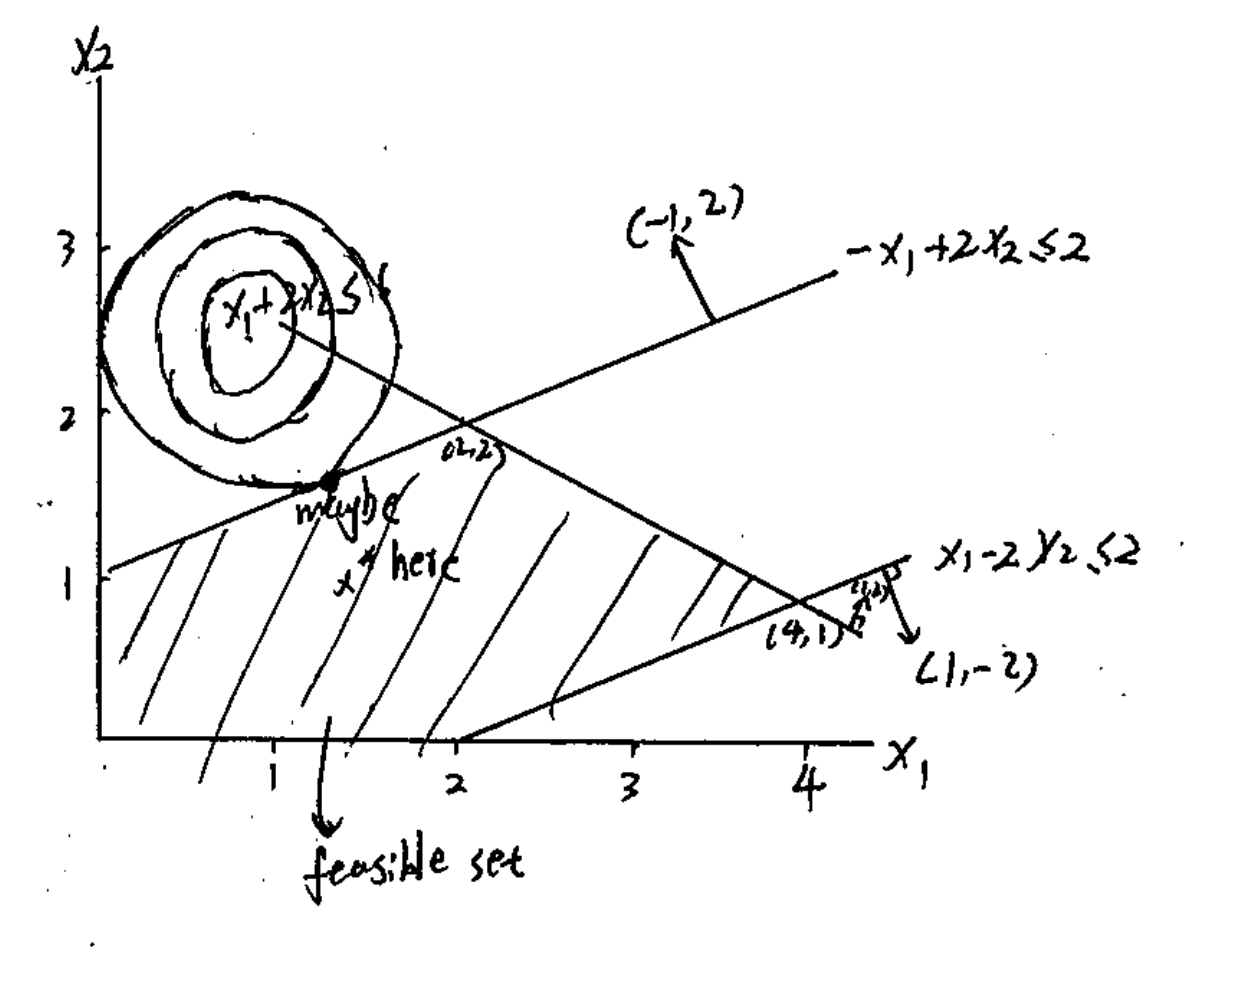
\includegraphics[width=1.8in,height=1.8in]{figures/ch07/figure1021_1.png}
	%\caption{This is an inserted JPG graphic} 
	%\label{fig:graph} 
\end{marginfigure}

\begin{itemize}
	\item at optimum some subset of inequality constraints satisfied with equality "active" set
	
	\item Best "loose"
	
	\item If you know the active set or optimum, just solve an "equality"-constrained QP"
\end{itemize}
By illustrative example:

1) Initialize at $x^{(0)} = \begin{bmatrix}
2\\
0
\end{bmatrix}$, starting with initial "working set" of equality constraint:

\begin{eqnarray}
w_0 = \{x|x_2 = 0 \}
\end{eqnarray}


2) \begin{equation*}
min_{x\in \Re^2} \frac{1}{2}x^T\begin{bmatrix}
2&0\\
0&2
\end{bmatrix}x + \begin{bmatrix}
-2 & -5
\end{bmatrix} + (1 + 2.5^2)
\end{equation*}

s.t. $\begin{bmatrix}
	0  & 1
\end{bmatrix}x = 0$

Recall from last time, we need a basis for $N(\begin{bmatrix}
0\\
1
\end{bmatrix}) = \{x|x = \alpha\begin{bmatrix}
0\\
1
\end{bmatrix} \}$

Say $\begin{bmatrix}
1\\
0
\end{bmatrix} = N\Leftarrow$

\begin{align*}
\tilde{H} &= N^THN = 2\\
\tilde{C} &= (c^TN + \bar{x}HN)\\
&= -2\tilde{d}\\
&= (d+c^Tx + \frac{1}{2}x^THx)
\end{align*}

We convert the problem to :

\begin{align*}
z^* &= argmin\,\,\, z^T\tilde{H}z + \tilde{c}^Tz + \tilde{d}\\
&= argmin\,\,\, \frac{1}{2}2z^2 + (-2z) = \tilde{d}
\end{align*}
 $2z - 2 = 0$, $z = 1$

So the optimum is:

\begin{equation*}
\bar{x}+ z^*N = \begin{bmatrix}
0\\
0
\end{bmatrix} + 1
\begin{bmatrix}
1\\
0
\end{bmatrix} = 
\begin{bmatrix}
1\\
0
\end{bmatrix}
\end{equation*}

Quadratically constrained Quadratic Program:

\begin{align*}
argmin_{x\in \Re^n} &\frac{1}{2}x^THx + c^T + d\\
s.t. &\frac{1}{2}x^TH_ix + c^T_i + d_i \leq 0  & i\in [m]\\
&\frac{1}{2}\tilde{H}_ix + \tilde{c}_i^Tx + \tilde{d}_i = 0 & i\in [q]
\end{align*}

\begin{itemize}
	\item If $H_i = 0, \forall i\in [n]$, $\tilde{H}_i = 0, \forall i\in [q]$, $\rightarrow QP$
	
	\item Typically $h-0\geq 0, H_i\geq 0$, $i\in [m], \tilde{H}_i = o, \forall i\in [q]$. "convex optimization program", set $\tilde{H}_i = 0$
\end{itemize}
Consider a single equality constraint $q = 1$, consider a scalar problem $x\in \Re$:

\begin{equation*}
\tilde{H}_1 = 1 \,\,\, \tilde{c}_i = 0 \,\,\, \tilde{d}_i = -\frac{1}{2}
\end{equation*}

Constraint becomes:

\begin{equation*}
\frac{1}{2}x_1^2 + 0 - \frac{1}{2} = 0\rightarrow x_1^2 = 1
\end{equation*}

Three types of inequality:

Type 1:

\begin{equation*}
H=\begin{bmatrix}
2 &\\
&\frac{1}{2}
\end{bmatrix}\,\,\,c^T = \begin{bmatrix}
0 & 0
\end{bmatrix}\,\,\,
d = -1
\end{equation*}

\begin{align*}
\frac{1}{2}x^THx + c^Tx + d \leq 0\Rightarrow &\frac{1}{2}x^T\begin{bmatrix}
2&\\
&\frac{1}{2}
\end{bmatrix}x\leq 1\\
&x^T\begin{bmatrix}
2&\\
&\frac{1}{2}
\end{bmatrix}x \leq 2
\end{align*}

\begin{align*}
2x_1^2 + \frac{1}{2}x_2^2 &\leq 2\\
x_1 + \frac{1}{4}x_2^2 &\leq 1\\
\frac{x_1^2}{1} + \frac{x_2^2}{4} &\leq 1
\end{align*}
Type 2:

\begin{equation*}
H=0\,\,\,c = \begin{bmatrix}
-1 & 1
\end{bmatrix}\,\,\,
d = -1
\end{equation*}
\begin{equation*}
\begin{bmatrix}
-1 & 1
\end{bmatrix}x\leq 1\Rightarrow
\begin{bmatrix}
-1 & 1
\end{bmatrix}
\begin{bmatrix}
x_1\\
x_2
\end{bmatrix}\leq 1\Rightarrow x_2\leq 1 + x_1
\end{equation*}

\begin{marginfigure}
	\centering
	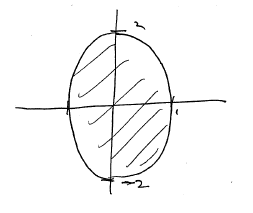
\includegraphics[width=1.8in,height=1.8in]{figures/ch07/figure1021_2.png}
	%\caption{This is an inserted JPG graphic} 
	%\label{fig:graph} 
\end{marginfigure}

Type 3:
\begin{equation*}
H=\begin{bmatrix}
0 &0\\
0&2
\end{bmatrix}\,\,\,c^T = \begin{bmatrix}
-1 & 0
\end{bmatrix}\,\,\,
d = -1 \Rightarrow x^2_2 - x_1 - 1\leq 0
\end{equation*}

\begin{marginfigure}
	\centering
	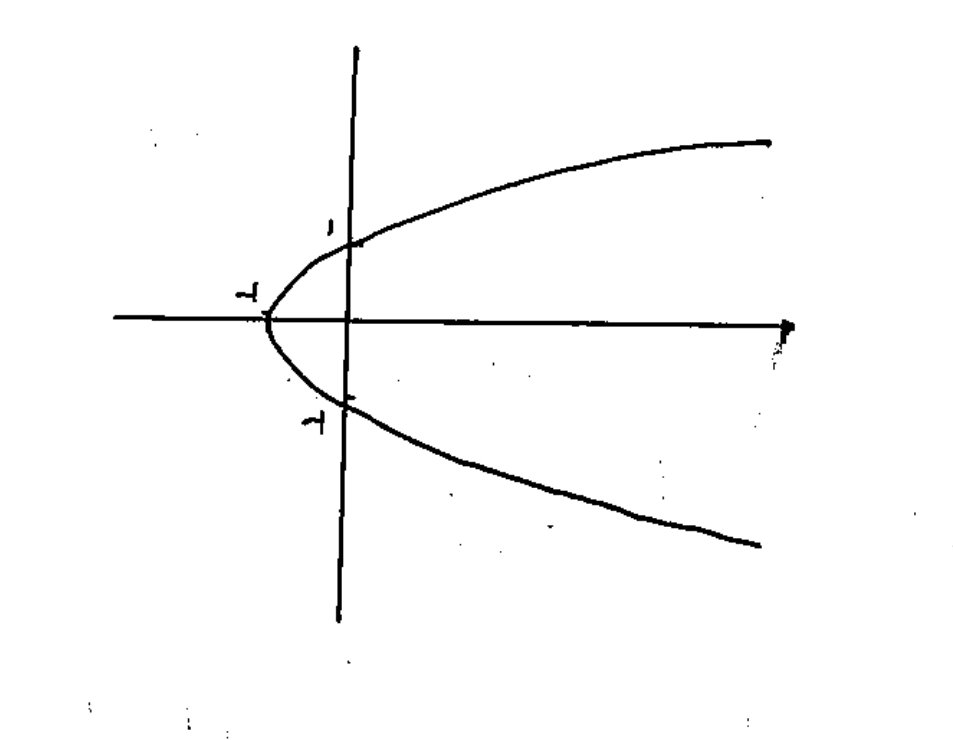
\includegraphics[width=1.8in,height=1.8in]{figures/ch07/figure1021_3.png}
	%\caption{This is an inserted JPG graphic} 
	%\label{fig:graph} 
\end{marginfigure}

Intersection:
\begin{marginfigure}
	\centering
	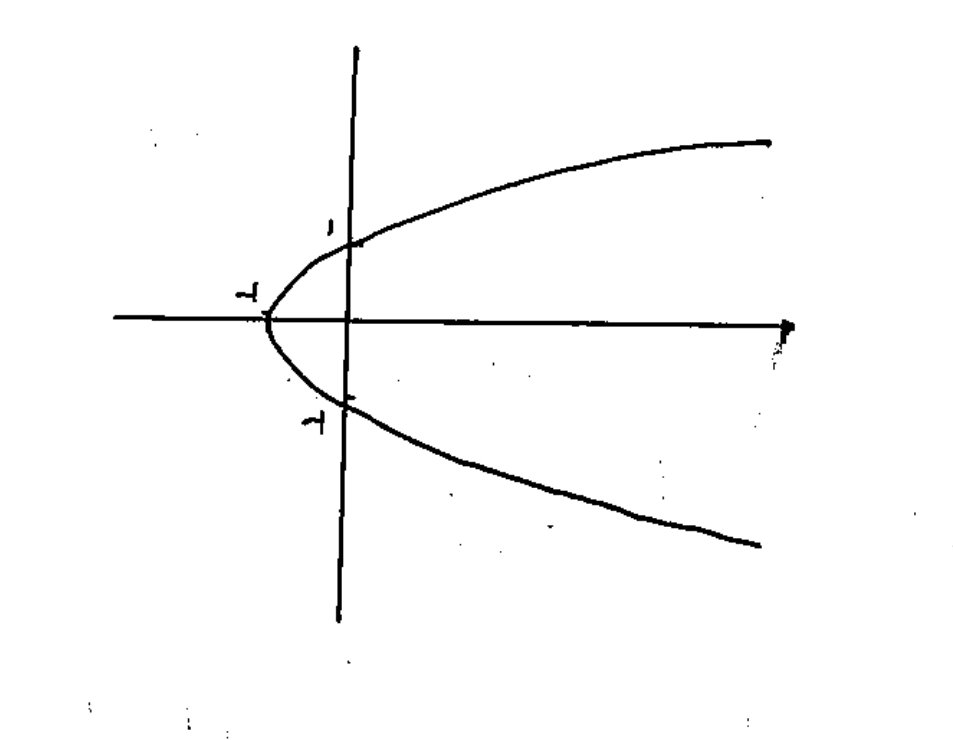
\includegraphics[width=1.8in,height=1.8in]{figures/ch07/figure1021_4.png}
	%\caption{This is an inserted JPG graphic} 
	%\label{fig:graph} 
\end{marginfigure}




%Above are notes for Oct21


%Below are notes for Oct21


%Above are notes for Oct23

